\documentclass{article}

\usepackage[final]{neurips_2025}
% The style file expects a track option alongside [final]; supply the default
% main-track notice string so the camera-ready footer resolves.
\makeatletter
\providecommand{\@trackname}{39th Conference on Neural Information Processing Systems (NeurIPS 2025).}
\makeatother

\usepackage[utf8]{inputenc}
\usepackage[T1]{fontenc}
\usepackage[hidelinks]{hyperref}
\usepackage{url}
\usepackage{booktabs}
\usepackage{graphicx}
\usepackage{amsmath,amssymb}
\usepackage{multirow}
\usepackage{enumitem}
\usepackage{caption}
\usepackage{subcaption}

% commands/general.tex customises algpseudocode spacing; define the hook so the
% file can be imported without loading the algorithm packages.
\providecommand{\algorithmicindent}{}

% Import command files
\input{commands/math}
\input{commands/general}
\input{commands/macros}

\captionsetup[table]{aboveskip=4pt,belowskip=4pt}
\captionsetup[figure]{aboveskip=4pt,belowskip=4pt}

\bibliographystyle{plainnat}

\title{Slow-Wave Sleep Stage Duration Is Not\\ Associated with Amyloid-Beta Burden:\\ A Cohort-Aware Meta-Analysis with a\\ Measurement-Reliability Null Model}

\author{NeuriCo}

\begin{document}

\maketitle

\begin{abstract}
The glymphatic hypothesis predicts that reduced slow-wave sleep permits amyloid-beta to
accumulate, and this prediction now drives trials that target N3 sleep duration as a route to
slowing Alzheimer's pathology. No meta-analysis has ever tested it: prior syntheses pooled
sleep quality, sleep duration or apnea severity, never a slow-wave-specific exposure against
amyloid PET. We pool 40 effect sizes from 17 studies and 12 cohort families, keeping N3
\emph{stage} amount strictly separate from \emph{spectral} slow-wave activity, aggregating
dependent effects to one synthetic effect per cohort family, and recovering correlations from
reported regression coefficients so that large cohorts are not silently dropped. The pooled
N3-stage/amyloid association is $r = +0.026$ (95\% CI $-0.153$ to $+0.203$, $p = 0.68$,
$I^2 = 0\%$), equivalence-tested tightly enough to reject a true correlation as large as
$r = 0.20$ ($p_{\mathrm{TOST}} = 0.026$). It is weaker, not stronger, than total sleep time
($r = +0.163$) and sleep efficiency ($r = +0.090$); all three preregistered specificity
contrasts point opposite to the hypothesis. We introduce a measurement-reliability null model
built from empirical single-night ICCs and show it predicts N3 should look $1.86\times$
\emph{stronger} than total sleep time; the observed ratio is $0.16\times$. Converted to the
hypothesis's own units, a 10-percentage-point reduction in N3 gives
$\Delta\mathrm{SUVR} = +0.005$, $1.8\%$ of the amyloid-negative/positive separation. The
positive spectral literature collapses from $r = +0.112$ to $r = -0.025$ when one cohort family
is removed.

\end{abstract}

\section{Introduction}
\label{sec:intro}

Sleep is one of very few \emph{modifiable} candidate risk factors for Alzheimer's disease, and
the glymphatic hypothesis gives it a concrete mechanism. Slow waves drive macroscopic
cerebrospinal-fluid pulsation in humans \citep{fultz2019}, that flow clears interstitial
amyloid-beta in mice \citep{xie2013}, and so chronically reduced slow-wave sleep should permit
amyloid to accumulate. The chain is repeated in reviews, in press coverage, and --- most
consequentially --- in the design of acoustic-stimulation and behavioural sleep trials that
treat N3 sleep duration as the actionable target. If the human evidence for the \emph{stage}
metric is weaker than the narrative implies, those trials are being powered and targeted on an
effect that may not exist at the claimed size.

\para{The hypothesis is a conjunction of three claims.} As usually stated, reduced slow-wave
sleep duration shows a dose-dependent association with higher amyloid burden in cognitively
normal adults, each 10\% reduction in N3 percentage is associated with a measurable increase in
amyloid PET SUVR, and this relationship is stronger than the associations with total sleep time
or sleep efficiency alone. Clause (i) is an association claim, clause (ii) a dose claim in
physical units, and clause (iii) a comparative claim. Each is separately testable, and the
hypothesis is supported only if all three hold.

\para{None of the three has ever been tested meta-analytically.} From 54 full-text papers we
find four gaps, and every one is load-bearing. First, no meta-analysis has pooled a
slow-wave-specific exposure against amyloid PET: the largest and most recent synthesis
\citep{chen2025} pooled only sleep \emph{quality} and \emph{duration} across 30 studies and
14{,}997 subjects, while \citet{cui2022} and \citet{bubu2020} covered obstructive sleep apnea.
Second, ``slow-wave sleep'' silently names two different measurements. In the one dataset that
reports both in the same 32 participants, spectral $<$1\,Hz slow-wave activity predicted amyloid
accumulation at $r = -0.52$ while N3 \emph{stage} duration was null at $r = -0.07$
\citep{winer2020}; any estimate that merges them is uninterpretable. Third, cohort
non-independence is unhandled: \citet{mander2015}, \citet{winer2019} and \citet{winer2020} are
all the Berkeley Aging Cohort Study with overlapping participants, contributing 13 of our 49
extracted effects. Fourth, and least appreciated, differential measurement reliability has
never been tested as a competing explanation for why one sleep metric correlates more strongly
than another.

\para{Our approach.} We assemble 49 hand-extracted effect sizes from 17 studies across 12
independent cohort families, each carrying a verified DOI/PMID, a verbatim provenance quote, and
a sign convention in which \emph{positive means worse sleep is associated with more amyloid}.
We pool the 40 amyloid-PET effects on the Fisher-$z$ scale in four preregistered strata ---
\stage, \spectral, \tst and \se{} --- aggregating to one synthetic effect per cohort family
before fitting REML random effects with Knapp--Hartung--Sidik--Jonkman standard errors. We then
test the comparative claim as a \emph{within-study paired difference} using only cohorts that
report both exposures in the same participants, build a measurement-reliability null model from
empirical single-night ICCs, and convert the pooled estimate into SUVR and Centiloid units
(\figref{fig:forest} through \figref{fig:robust}).

\para{What we find.} The exposure the hypothesis names is the weakest of the four:
$r = +0.026$ (95\% CI $-0.153$ to $+0.203$, $p = 0.68$) with $I^2 = 0\%$, against $r = +0.163$
for total sleep time and $r = +0.090$ for sleep efficiency. Equivalence testing rejects a true
correlation as large as $r = 0.20$ ($p_{\mathrm{TOST}} = 0.026$). The dose statement converts to
$\Delta\mathrm{SUVR} = +0.005$ per 10 \pp of N3, $1.8\%$ of the amyloid-negative/positive
separation. Measurement error cannot rescue the comparative claim: single-night polysomnography
measures N3\% far more reliably (ICC $0.775$) than total sleep time (ICC $0.225$), so identical
true effects would still make N3 look $1.86\times$ stronger --- the observed ratio is
$0.16\times$, about eleven times below the measurement-only prediction. Finally, the positive
spectral literature is one cohort family: pooled $r = +0.112$ across three families
($I^2 = 77\%$) drops to $r = -0.025$ when Berkeley is removed.

\para{Contributions.}
\begin{itemize}[leftmargin=*,itemsep=1pt,topsep=2pt]
    \item We provide the first meta-analytic estimate of the N3-stage/amyloid-PET association,
    kept strictly separate from spectral slow-wave activity and with variance handled at the
    level of the cohort family rather than the publication.
    \item We test the specificity claim as a within-study paired contrast, using only cohorts
    that measure both exposures in the same participants, which removes between-cohort
    confounding from the exact comparison the hypothesis makes.
    \item We introduce a quantitative measurement-reliability null model from empirical
    single-night ICCs, turning ``metric A correlates more strongly than metric B'' into a
    testable excess over what measurement precision alone predicts.
    \item We estimate the hypothesis's own dose statement in SUVR and Centiloid units, and show
    with population N3 distributions that the stated 10-percentage-point contrast is not
    available to 78\% of the target population.
\end{itemize}

\Secref{sec:related} positions this work against the mechanistic, observational and
meta-analytic literature; \secref{sec:method} gives the harmonisation, dependency handling and
six preregistered analyses; \secref{sec:results} reports them; \secref{sec:discussion} states
the verdict on each clause, what the reliability model adds, and the limits of a study-level
design.

\section{Related Work}
\label{sec:related}

\para{Mechanism: why anyone expects an effect.} \citet{xie2013} showed that convective
interstitial-fluid exchange increases during natural sleep and anaesthesia in mice, with a
roughly 60\% increase in interstitial space and faster clearance of exogenous amyloid-beta.
\citet{fultz2019} supplied the human counterpart: during NREM sleep, coupled
electrophysiological, haemodynamic and CSF oscillations produce large macroscopic CSF flow
pulsations locked to slow-wave activity. \citet{holth2019} extended the same logic to tau, and
\citet{rasmussen2018} review the pathway across neurological disease. The closest thing to a
human experiment is \citet{ju2017}: in 17 adults, acoustic disruption of slow-wave activity
raised CSF amyloid-beta40 ($r = 0.610$, $p = 0.009$), and the authors report the effect as
specific to slow-wave activity rather than to sleep duration or efficiency. Unlike that work,
which measures the acute overnight production/clearance balance in soluble CSF, we ask whether
chronically lower slow-wave sleep is visible in \emph{deposited} plaque on PET.

\para{Spectral slow-wave activity and amyloid.} \citet{mander2015} reported that the proportion
of medial-prefrontal NREM slow-wave activity in the 0.6--1\,Hz band correlated with mPFC PiB DVR
at $r = -0.45$, with the effect frequency-specific: the 1--4\,Hz band trended the other way.
\citet{winer2019} replicated this at $r = -0.36$ (rising to $-0.43$ adjusted), and
\citet{winer2020} showed prospectively that baseline $<$1\,Hz slow-wave activity predicted the
rate of subsequent cortical amyloid accumulation at $r = -0.52$. All three draw on the Berkeley
Aging Cohort Study with overlapping participants. Two independent attempts did not reproduce
the finding: \citet{champetier2024} decomposed delta into sub-bands in 127 cognitively
unimpaired adults and found no association with amyloid at baseline or with accumulation, and
\citet{carvalho2024} found slow-oscillation relative power \emph{increased} annualised PiB
accumulation in older adults with apnea. \citet{lucey2019} report the inverse relation most
strongly for tau rather than amyloid, and \citet{zavecz2023} reframe slow-wave activity as a
cognitive-reserve factor that moderates the effect of amyloid on memory rather than predicting
amyloid level itself. Building on this literature, we do not merge these
effects with stage-level ones, and we quantify how much of the pooled spectral estimate rests
on a single cohort family.

\para{Stage-level slow-wave sleep.} The metric the hypothesis actually names --- N3 stage
duration or percentage --- has a much flatter record. \citet{montagne2026} found N3\% did not
differ by amyloid status in 76 cognitively unimpaired adults ($\eta_p^2 = 0.003$, $p = 0.628$)
while total sleep time did ($\eta_p^2 = 0.065$, $p = 0.031$). \citet{jin2025} found slow-wave
sleep tertiles null against amyloid PET in fully adjusted models, with REM latency rather than
slow-wave sleep carrying the association. \citet{stankeviciute2024} tie decreased slow-wave
sleep to tau rather than amyloid and report the associations as amyloid-independent.
\citet{varga2016} and \citet{liguori2020} use CSF amyloid-beta42 rather than PET, and their
signs relative to deposited burden are opposite because their samples sit on opposite sides of
deposition. We treat CSF as a cognitive-status-stratified secondary rather than pooling it with
PET.

\para{Duration and efficiency: the comparators the hypothesis must beat.} \citet{winer2021}
found shorter self-reported sleep associated with higher amyloid in 4{,}417 A4 screening
participants; \citet{spira2013} reported the same direction in the BLSA neuroimaging substudy;
\citet{insel2021} found null global effects in A4 with regional effects only for daytime sleep;
\citet{pivac2024} linked low sleep efficiency to faster accumulation in AIBL; \citet{brown2016}
found only sleep latency significant among PSQI components; and \citet{fenton2023} found
actigraphic \emph{variability} in efficiency and duration predicted burden. These are the
field's de-facto comparators, and clause (iii) of the hypothesis is precisely the claim that
slow-wave sleep beats them.

\para{Prior meta-analyses.} \citet{chen2025} is the largest synthesis to date and pools poor
sleep quality against amyloid PET at Fisher $z = 0.153$ ($k = 9$, $I^2 = 99\%$).
\citet{bubu2019} and \citet{bubu2020} cover apnea and longitudinal biomarker change, and
\citet{cui2022} meta-analyses AD biomarkers in apnea. None pools a slow-wave-specific exposure.
We also note a metric defect in the benchmark: \citet{chen2025} report ``Fisher $z = -0.002$,
95\% CI $-0.003$ to $-0.001$'' for sleep duration against amyloid PET, which are raw
regression-coefficient units labelled as Fisher $z$; a pooled correlation of $-0.002$ with that
interval is not a credible common metric. Our pipeline converts every input to a genuinely
common metric before pooling, and we report the conversion rule for each effect.

\para{Measurement and reference scales.} Night-to-night variability in sleep-stage measurement
is well documented \citep{levendowski2017}, as are the limits of inter-scorer agreement
\citep{nikkonen2024}, but no paper in our corpus asks whether metric-to-metric differences in
\emph{observed} correlation strength follow from metric-to-metric differences in single-night
reliability. We make that question quantitative. For unit conversion we use the amyloid PET
reference distributions and the 1.42\,SUVR / 19\,Centiloid positivity threshold of
\citet{jack2017}, with \citet{hanseeuw2021} for progression anchors, and we take single-night
reliabilities from \sleepedf \citep{kemp2000}. Our meta-analytic machinery follows
\citet{viechtbauer2005} for REML, \citet{knapp2003} for small-sample standard errors,
\citet{higgins2009} for prediction intervals, \citet{borenstein2009} for correlated-effects
aggregation, \citet{hedges2010} for cluster-robust variance, \citet{egger1997} and
\citet{duval2000} for small-study bias, and \citet{lakens2017} for equivalence testing.

\section{Methodology}
\label{sec:method}

\subsection{The hypothesis, decomposed into testable clauses}
\label{sec:clauses}

We preregistered the hypothesis as a conjunction and fixed a refutation criterion for each
clause before fitting any model (\tabref{tab:clauses}). Clause (i) is tested by the pooled
association and, if null, by equivalence testing; clause (ii) by conversion to
$\Delta\mathrm{SUVR}$ per 10 \pp of N3; clause (iii) by within-study paired contrasts that must
additionally survive a measurement-reliability null model. A negative result on any clause is
reported as the finding.

\begin{table}[t]
    \centering
    \small
    \begin{tabular}{@{}cp{2.9cm}p{3.5cm}p{4.5cm}@{}}
        \toprule
        \textbf{Clause} & \textbf{Claim} & \textbf{Supported if} & \textbf{Refuted if} \\
        \midrule
        (i)   & N3 stage \% is associated with amyloid PET burden
              & pooled $r > 0$ with 95\% CI excluding 0
              & CI includes 0 \emph{and} excludes $r \geq 0.20$ (TOST) \\
        (ii)  & the association is dose-dependent and measurable in SUVR
              & $\Delta\mathrm{SUVR}$ per 10 \pp CI excludes 0 and is a non-trivial fraction of
                the A$-$/A$+$ separation
              & CI includes 0, \emph{or} magnitude $< \sim$5\% of the A$-$/A$+$ SUVR gap \\
        (iii) & it is \emph{stronger} than \tst and \se
              & paired $\Delta z > 0$ with CI excluding 0 \emph{and} the excess survives the
                reliability null
              & $\Delta z \leq 0$, \emph{or} any positive gap is fully explained by differential
                ICC \\
        \bottomrule
    \end{tabular}
    \caption{The hypothesis decomposed into three preregistered clauses with their refutation
    criteria, fixed before any model was fitted. The hypothesis is a conjunction: it is
    supported only if all three clauses hold.}
    \label{tab:clauses}
\end{table}


\subsection{Corpus and analysis set}
\label{sec:data}

The primary input is a curated table of 49 effect sizes hand-extracted from 17 studies across 12
independent cohort families. Every row carries a verified DOI or PMID, a verbatim provenance
quote from the source paper, a \texttt{cohort\_family} label used for dependency handling, and a
\emph{burden-aligned} effect signed so that \textbf{positive means worse sleep is associated
with more amyloid}. Positive therefore always supports the hypothesis, regardless of how the
original paper oriented its exposure.

The primary analysis set is the 40 usable effects whose outcome is amyloid PET burden
(cross-sectional deposition or change). The nine CSF amyloid-beta42 effects are excluded from
the primary model and analysed only as a cognitive-status-stratified secondary, because the sign
of soluble CSF amyloid-beta42 relative to deposited burden reverses between pre-deposition
samples \citep{varga2016} and post-deposition samples \citep{liguori2020}.

Three supporting datasets do the work the primary table cannot. Single-night ICC(2,1) values per
sleep metric come from \sleepedf \citep{kemp2000}, computed on 75 subjects with two consecutive
nights each, and feed the reliability null model. Subject-level N3 percentages from the same
source (153 recordings, 78 subjects) give the exposure dispersion for the dose conversion and
the feasibility check. Amyloid SUVR/Centiloid anchors come from \citet{jack2017}, and
\citet{chen2025} serves as an external benchmark for the pooled comparator estimates.

\subsection{Effect harmonisation}
\label{sec:harmonise}

Everything is pooled on the Fisher-$z$ scale \citep{fisher1915},
$z = \operatorname{artanh}(r)$ with $v = 1/(n-3)$. Kendall's $\tau$ is converted through
Greiner's relation $r = \sin(\pi\tau/2)$ \citep{kendall1949}. \Tabref{tab:conversion} lists the conversion rule applied to each input type and
how many amyloid-PET effects it covers.

\begin{table}[t]
    \centering
    \small
    \resizebox{\ifdim\width>\textwidth\textwidth\else\width\fi}{!}{%
\begin{tabular}{@{}llc@{}}
        \toprule
        \textbf{Input type} & \textbf{Conversion rule} & \textbf{PET effects} \\
        \midrule
        \texttt{pearson\_r}, \texttt{partial\_r}, \texttt{r\_from\_partial\_eta2}
            & used directly as $r$ (with $r = \sqrt{\eta_p^2}$ for a 1-df contrast) & 20 \\
        \texttt{kendall\_tau}
            & $r = \sin(\pi\tau/2)$ (Greiner's relation) & 1 \\
        \texttt{unstd\_beta\_*}
            & test-statistic recovery, \eqref{eq:recovery} & 12 \\
        \texttt{narrative\_null}
            & imputed $z = 0$, $v = 1/(n-3)$ & 7 \\
        \midrule
        \multicolumn{2}{@{}l}{\textbf{Total usable amyloid-PET effects}} & \textbf{40} \\
        \bottomrule
    \end{tabular}%
}
    \caption{Effect harmonisation rules, fixed in advance and applied uniformly. All effects are
    pooled as Fisher $z$ with $v = 1/(n-3)$. Test-statistic recovery raises the usable
    amyloid-PET set from 21 native correlations to 40 effects and is what brings the two largest
    cohorts onto the common metric.}
    \label{tab:conversion}
\end{table}


\para{Test-statistic recovery.} The step that makes this analysis possible is the recovery of a
partial correlation from a reported regression coefficient and its $p$-value
\citep{rosenthal1979}. For a two-sided $p$ on $\mathrm{df} = n - 1 - n_{\mathrm{cov}}$ residual
degrees of freedom,
\begin{equation}
t = \operatorname{sign}(\beta)\, F^{-1}\!\left(1 - \tfrac{p}{2};\, \mathrm{df}\right),
\qquad
r = \frac{t}{\sqrt{t^{2} + \mathrm{df}}}.
\label{eq:recovery}
\end{equation}
Raw betas are never pooled in their native units. Recovery brings the two largest cohorts
(\afour, $n = 4{,}417$; \aibl, $n = 189$) and the \mayo and \mars results onto the common
metric, raising the usable amyloid-PET set from 21 native correlations to 40 effects. The
conversion is exact where it can be checked: recovering $r$ from the $p$-value of a simple
correlation returns the original $r$ to within $10^{-8}$.

\para{Reported nulls.} Seven amyloid-PET effects are narrative nulls --- statements such as ``no
association with total sleep time or sleep efficiency'' with no number attached. We impute
$z = 0$ with $v = 1/(n-3)$. This is conservative in magnitude but anti-conservative in
precision, so it is carried as the primary rule \emph{and} removed in sensitivity analysis S1.
Dropping these rows instead would bias every pooled estimate away from zero.

\subsection{Dependency handling and estimation}
\label{sec:estimation}

Berkeley alone contributes 13 of 49 effects, so treating publications as independent would
inflate precision. The primary estimator first aggregates to one synthetic effect per cohort
family per stratum using the correlated-effects variance of \citet{borenstein2009},
\begin{equation}
\bar{z} = \frac{1}{m}\sum_{i=1}^{m} z_i,
\qquad
\bar{v} = \frac{1}{m^{2}}\left(\sum_{i=1}^{m} v_i + \sum_{i \neq j} \rho \sqrt{v_i v_j}\right),
\qquad \rho = 0.6,
\label{eq:borenstein}
\end{equation}
and then fits REML random effects \citep{viechtbauer2005} with
Knapp--Hartung--Sidik--Jonkman standard errors on a $t_{k-1}$ reference distribution
\citep{knapp2003}, the recommended small-$k$ adjustment. Naive per-effect pooling is reported
only to quantify how much dependency handling matters, and cluster-robust variance estimation
\citep{hedges2010} is reported where a stratum has at least four cohort families.

\subsection{The six analyses}
\label{sec:experiments}

\para{E1: stratified pooling.} Pooled estimates for \stage, \spectral, \tst, \se, \waso and
other stages, with $\tau^2$, $Q$, $I^2$ and a 95\% prediction interval \citep{higgins2009}.
Because $k \leq 6$ cohort families per stratum, every primary $p$-value is accompanied by an
exact sign-flip permutation $p$-value enumerating all $2^k$ assignments.

\para{E2: specificity.} A naive between-stratum comparison is invalid because the strata share
cohorts. The primary test is therefore a within-study paired difference: for every cohort family
reporting both exposures in the same participants,
$\Delta z = z_{\mathrm{N3}} - z_{\mathrm{comparator}}$ with
$\operatorname{Var}(\Delta z) = v_a + v_b - 2\rho_w\sqrt{v_a v_b}$ and $\rho_w = 0.5$. Three
preregistered confirmatory contrasts (stage vs.\ \tst, stage vs.\ \se, stage vs.\ \spectral)
carry a Holm correction \citep{holm1979}.

\para{E3: measurement-reliability null model.} Classical attenuation gives
$r_{\mathrm{obs}} = r_{\mathrm{true}}\sqrt{\mathrm{ICC}_{\mathrm{exposure}}}
\sqrt{\mathrm{ICC}_{\mathrm{outcome}}}$. In a within-outcome comparison the outcome term
cancels, so if two exposures had \emph{identical} true correlations with amyloid their observed
correlations would still stand in the ratio
$\sqrt{\mathrm{ICC}_a / \mathrm{ICC}_b}$. We compute that predicted ratio from the empirical
single-night ICCs and compare it to the observed ratio, and we also report each stratum
disattenuated for its own unreliability.

\para{E4: dose conversion and feasibility.} We convert the pooled correlation into the units the
hypothesis states,
\begin{equation}
\Delta\mathrm{amyloid} \text{ per } 10\,\mathrm{pp\ N3}
= r_{\mathrm{pooled}} \times \frac{10}{\mathrm{SD}_{\mathrm{N3\%}}}
\times \mathrm{SD}_{\mathrm{amyloid}},
\label{eq:dose}
\end{equation}
propagating all three inputs by Monte Carlo (10{,}000 draws): $r$ via a $t_{k-1}$ draw on the
Fisher-$z$ scale, $\mathrm{SD}_{\mathrm{N3\%}}$ via the $\chi^2$ sampling distribution of an SD,
and $\mathrm{SD}_{\mathrm{amyloid}}$ via a $\mathrm{Beta}(30,70)$ prior on amyloid-positive
prevalence applied to the medians and IQRs of \citet{jack2017}. We then ask whether a
10-percentage-point reduction in N3 is an available exposure contrast at all, using the observed
N3 distribution in \sleepedf subjects aged 60 and over.

\para{E5: robustness and bias.} Seventeen preregistered specifications: dropping imputed nulls
(S1), dropping $p$-recovered betas (S2), both (S1+S2), alternative residual-df rules (S3),
$\rho \in \{0.3, 0.8, 1.0\}$ (S4), cognitively normal samples only (S5), PSG-measured exposures
only (S6), leave-one-cohort-family-out (S7), fixed effects (S8), and the CSF secondary (S10).
Small-study bias by Egger regression \citep{egger1997} and Duval--Tweedie trim-and-fill
\citep{duval2000}, labelled uninterpretable below $k = 5$ and $k = 10$ respectively.

\para{E6: precision.} Minimum detectable effect at 80\% power per stratum, power at
$r \in \{0.20, 0.30, 0.45\}$, and equivalence testing \citep{lakens2017} of the \stage stratum
against bounds $r = \pm 0.10, 0.15, 0.20, 0.30, 0.45$. An honest negative result must state what
it could and could not have detected.

\subsection{Implementation and reproducibility}
\label{sec:impl}

Python 3.12.8 with numpy 2.5.2, pandas 3.0.5, scipy 1.18.1, statsmodels 0.15.0 and pymare
0.0.12, in an isolated \texttt{uv} environment with pinned dependencies. Seed 42 throughout;
the only stochastic step is the E4 Monte Carlo. The full pipeline runs in about 29 seconds on
CPU. GPUs were available but not used: this is a study-level meta-analysis whose entire compute
cost is trivial, so acceleration would add complexity with no benefit.

The meta-analytic primitives (REML $\tau^2$, HKSJ, cluster-robust variance, exact permutation,
trim-and-fill, TOST) are implemented directly from their primary formulations rather than taken
from a package, because no available Python package provides HKSJ, cluster-robust variance and
exact permutation together. They are cross-checked against PyMARE, an independently maintained
meta-analysis package: REML point estimates agree to within $4.4 \times 10^{-9}$ on all four
strata. Validation re-runs the entire pipeline in a scratch copy and confirms all eight result
files are bit-identical; 39 of 39 validation checks pass.

\section{Results}
\label{sec:results}

\begin{figure}[t]
    \centering
    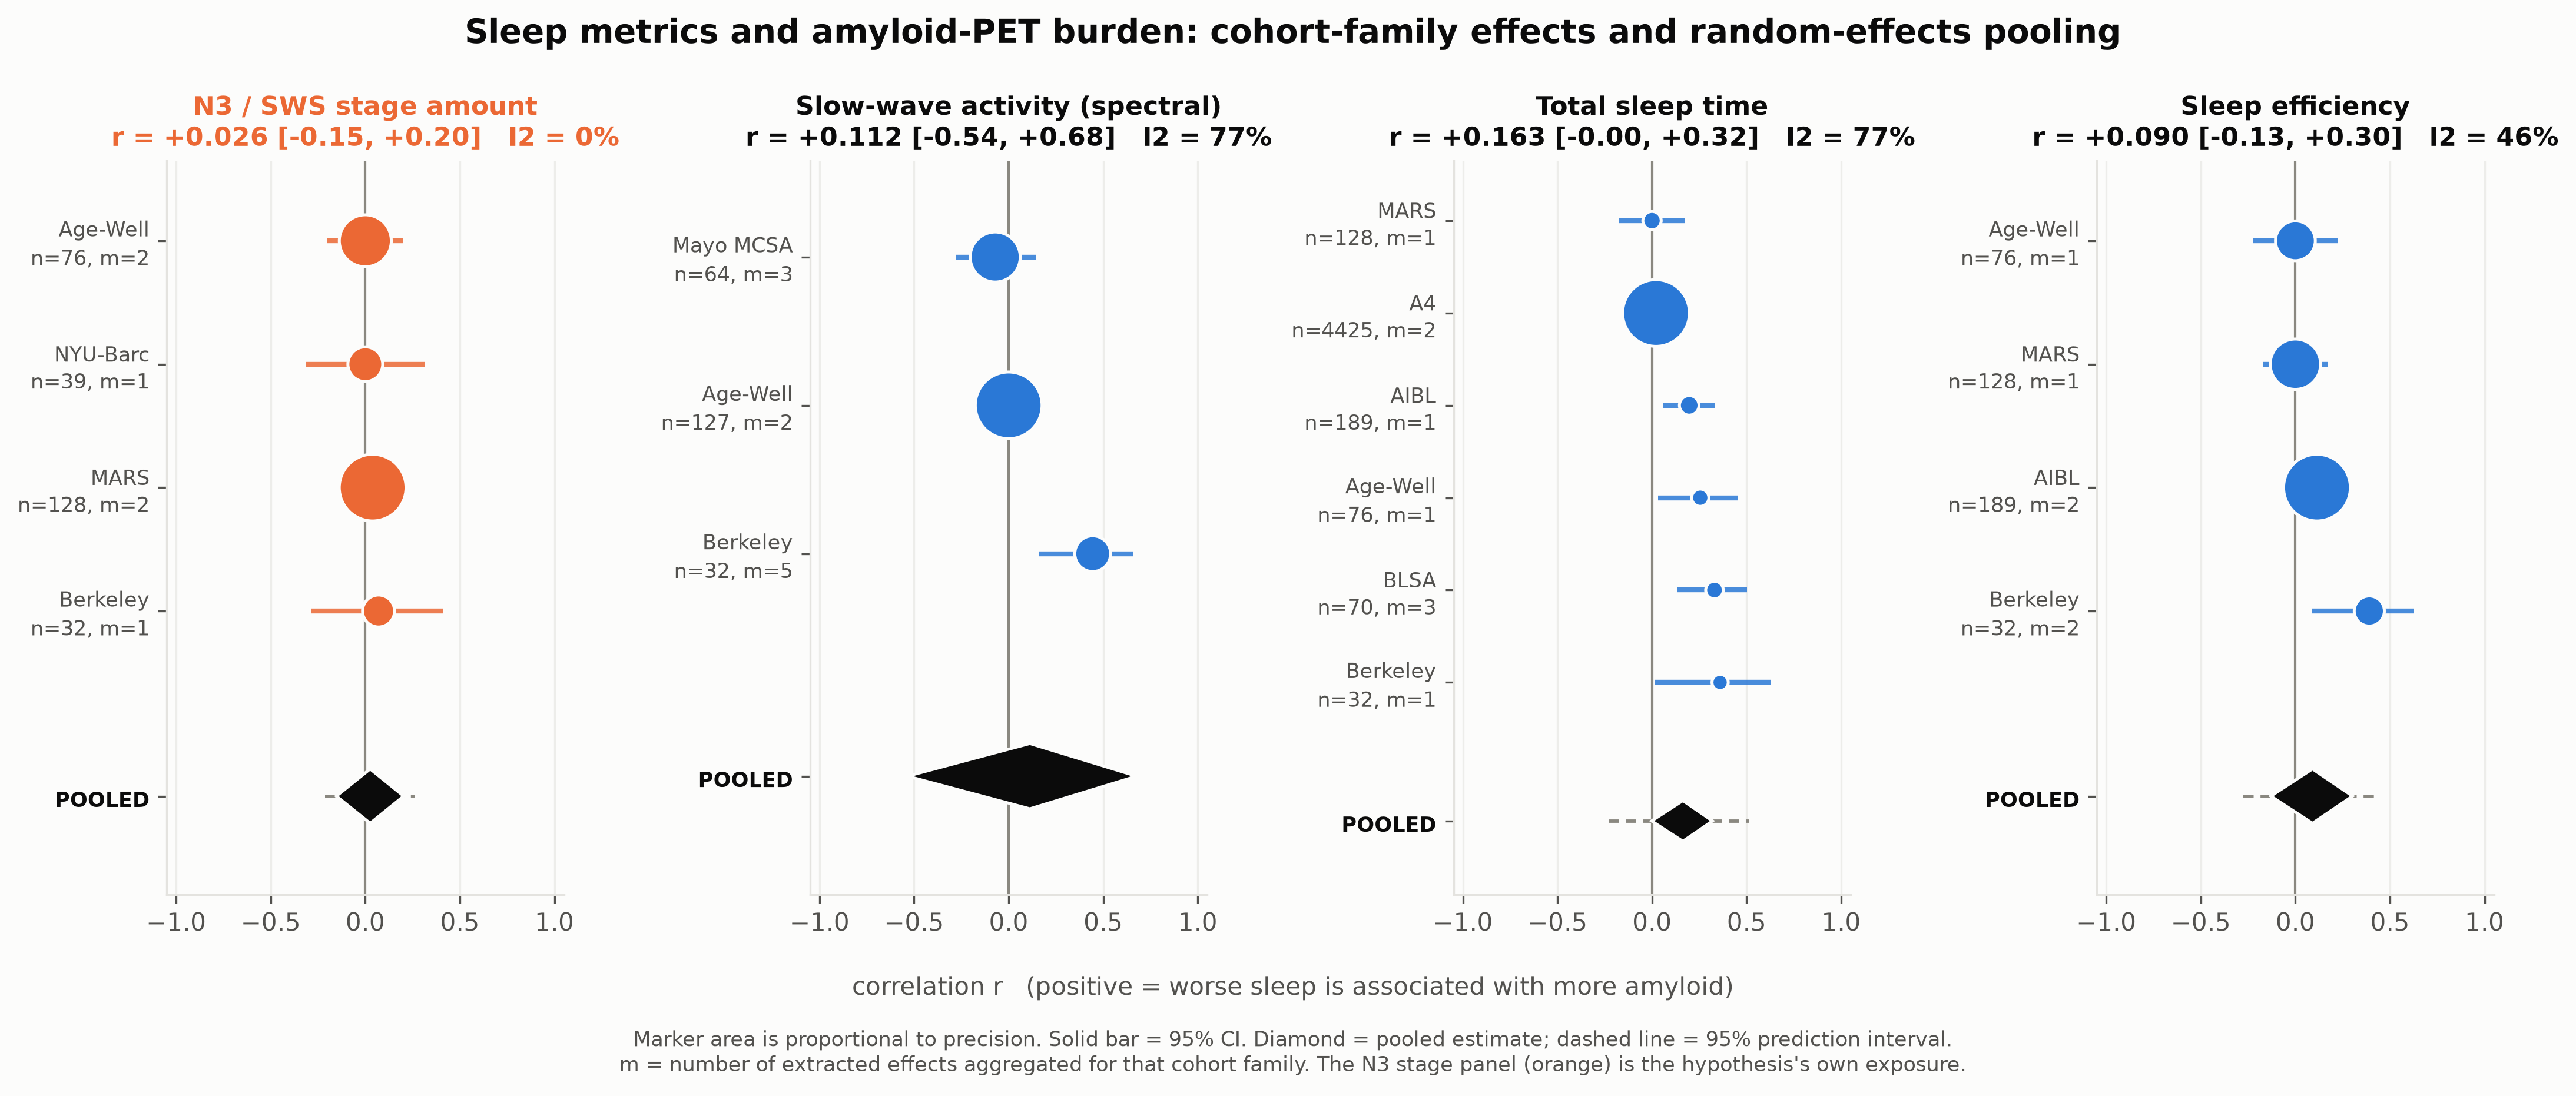
\includegraphics[width=\linewidth]{figures/fig1_forest_by_stratum.png}
    \caption{E1: cohort-family effects and random-effects pooling for the four preregistered
    exposures. Marker area is proportional to precision, solid bars are 95\% CIs, diamonds are
    pooled estimates and dashed lines are 95\% prediction intervals; $m$ is the number of
    extracted effects aggregated for that cohort family. Positive $r$ means worse sleep is
    associated with more amyloid. The hypothesis's own exposure (\stage, orange, leftmost) is the
    weakest and the most homogeneous: four independent cohort families agree there is nothing
    there. \spectral is the opposite case --- \berkeley at $r = +0.44$ against \mayo at $-0.07$
    and \agewell at $0.00$.}
    \label{fig:forest}
\end{figure}

\begin{table}[t]
    \centering
    \resizebox{\ifdim\width>\textwidth\textwidth\else\width\fi}{!}{%
    \begin{tabular}{@{}lccrcccccc@{}}
        \toprule
        \textbf{Exposure} & \textbf{$k$ eff.} & \textbf{cohorts} & \textbf{$\Sigma n$} &
        \textbf{pooled $r$} & \textbf{95\% CI} & \textbf{$p$} & \textbf{perm.\ $p$} &
        \textbf{$\tau^2$} & \textbf{$I^2$} \\
        \midrule
        \stage \textit{(the hypothesis's exposure)} & 6 & 4 & 275 & $\mathbf{+0.026}$ & $[-0.153, +0.203]$ & 0.68 & 0.50 & 0.000 & \phantom{0}0\% \\
        \spectral                                   & 10 & 3 & 223 & $+0.112$ & $[-0.535, +0.677]$ & 0.57 & 1.00 & 0.062 & 77\% \\
        \tst                                        & 9 & 6 & 4{,}920 & $\mathbf{+0.163}$ & $[-0.002, +0.320]$ & 0.052 & 0.062 & 0.016 & 77\% \\
        \se                                         & 6 & 4 & 425 & $+0.090$ & $[-0.130, +0.302]$ & 0.28 & 0.50 & 0.003 & 46\% \\
        \midrule
        \waso                                       & 2 & 2 & 108 & $+0.109$ & $[-0.975, +0.984]$ & 0.65 & 1.00 & 0.043 & 64\% \\
        Other stages (N1/N2/REM)                    & 4 & 2 & 108 & $+0.198$ & $[-0.728, +0.868]$ & 0.26 & 0.50 & 0.000 & \phantom{0}0\% \\
        \bottomrule
    \end{tabular}%
    }
    \caption{E1: pooled associations between each sleep metric and amyloid PET burden. Positive
    $r$ means \emph{worse sleep is associated with more amyloid}, so positive supports the
    hypothesis. Estimates are REML random effects with HKSJ standard errors on one synthetic
    effect per cohort family. The exposure the hypothesis names (\stage) is the weakest of the
    four preregistered strata and the only one with zero heterogeneity; the largest estimate
    belongs to \tst, which the hypothesis predicts should be weaker. Permutation $p$-values
    enumerate all $2^k$ sign flips of the cohort-level effects.}
    \label{tab:pooled}
\end{table}


\subsection{E1: the exposure the hypothesis names is the weakest of the four}
\label{sec:e1}

\Tabref{tab:pooled} and \figref{fig:forest} give the primary estimates. The pooled association
between N3 stage amount and amyloid PET burden is $r = +0.026$ (95\% CI $-0.153$ to $+0.203$,
$p = 0.68$, permutation $p = 0.50$) across 6 effects from 4 independent cohort families. Its
heterogeneity is zero ($I^2 = 0\%$, $\tau^2 = 0.000$) and its prediction interval is tight
($-0.21$ to $+0.26$): the cohort families agree with each other. Cluster-robust variance
estimation gives essentially the same answer wherever it is interpretable --- for \tst with six
clusters, $r = 0.160$ (95\% CI $-0.002$ to $0.313$, $p = 0.052$).

The ordering is the reverse of what the hypothesis predicts. \tst is the strongest stratum at
$r = +0.163$ ($p = 0.052$) across six cohort families and $\Sigma n = 4{,}920$, and \se is
$+0.090$; both exceed the exposure that is supposed to beat them. The spectral stratum sits at
$r = +0.112$ but with $I^2 = 77\%$ and a prediction interval spanning the entire correlation
scale, which is a statement about disagreement rather than about effect size.

Our \tst estimate is a useful external check. \citet{chen2025} independently pooled sleep
quality against amyloid PET at Fisher $z = 0.153$ ($r = 0.152$, $k = 9$, $n = 10{,}132$); our
$r = 0.163$ is the same order, which is reassuring evidence that the harmonisation pipeline
produces sane numbers on a stratum where an external benchmark exists.

\subsection{E2: all three specificity contrasts point the wrong way}
\label{sec:e2}

\begin{figure}[t]
    \centering
    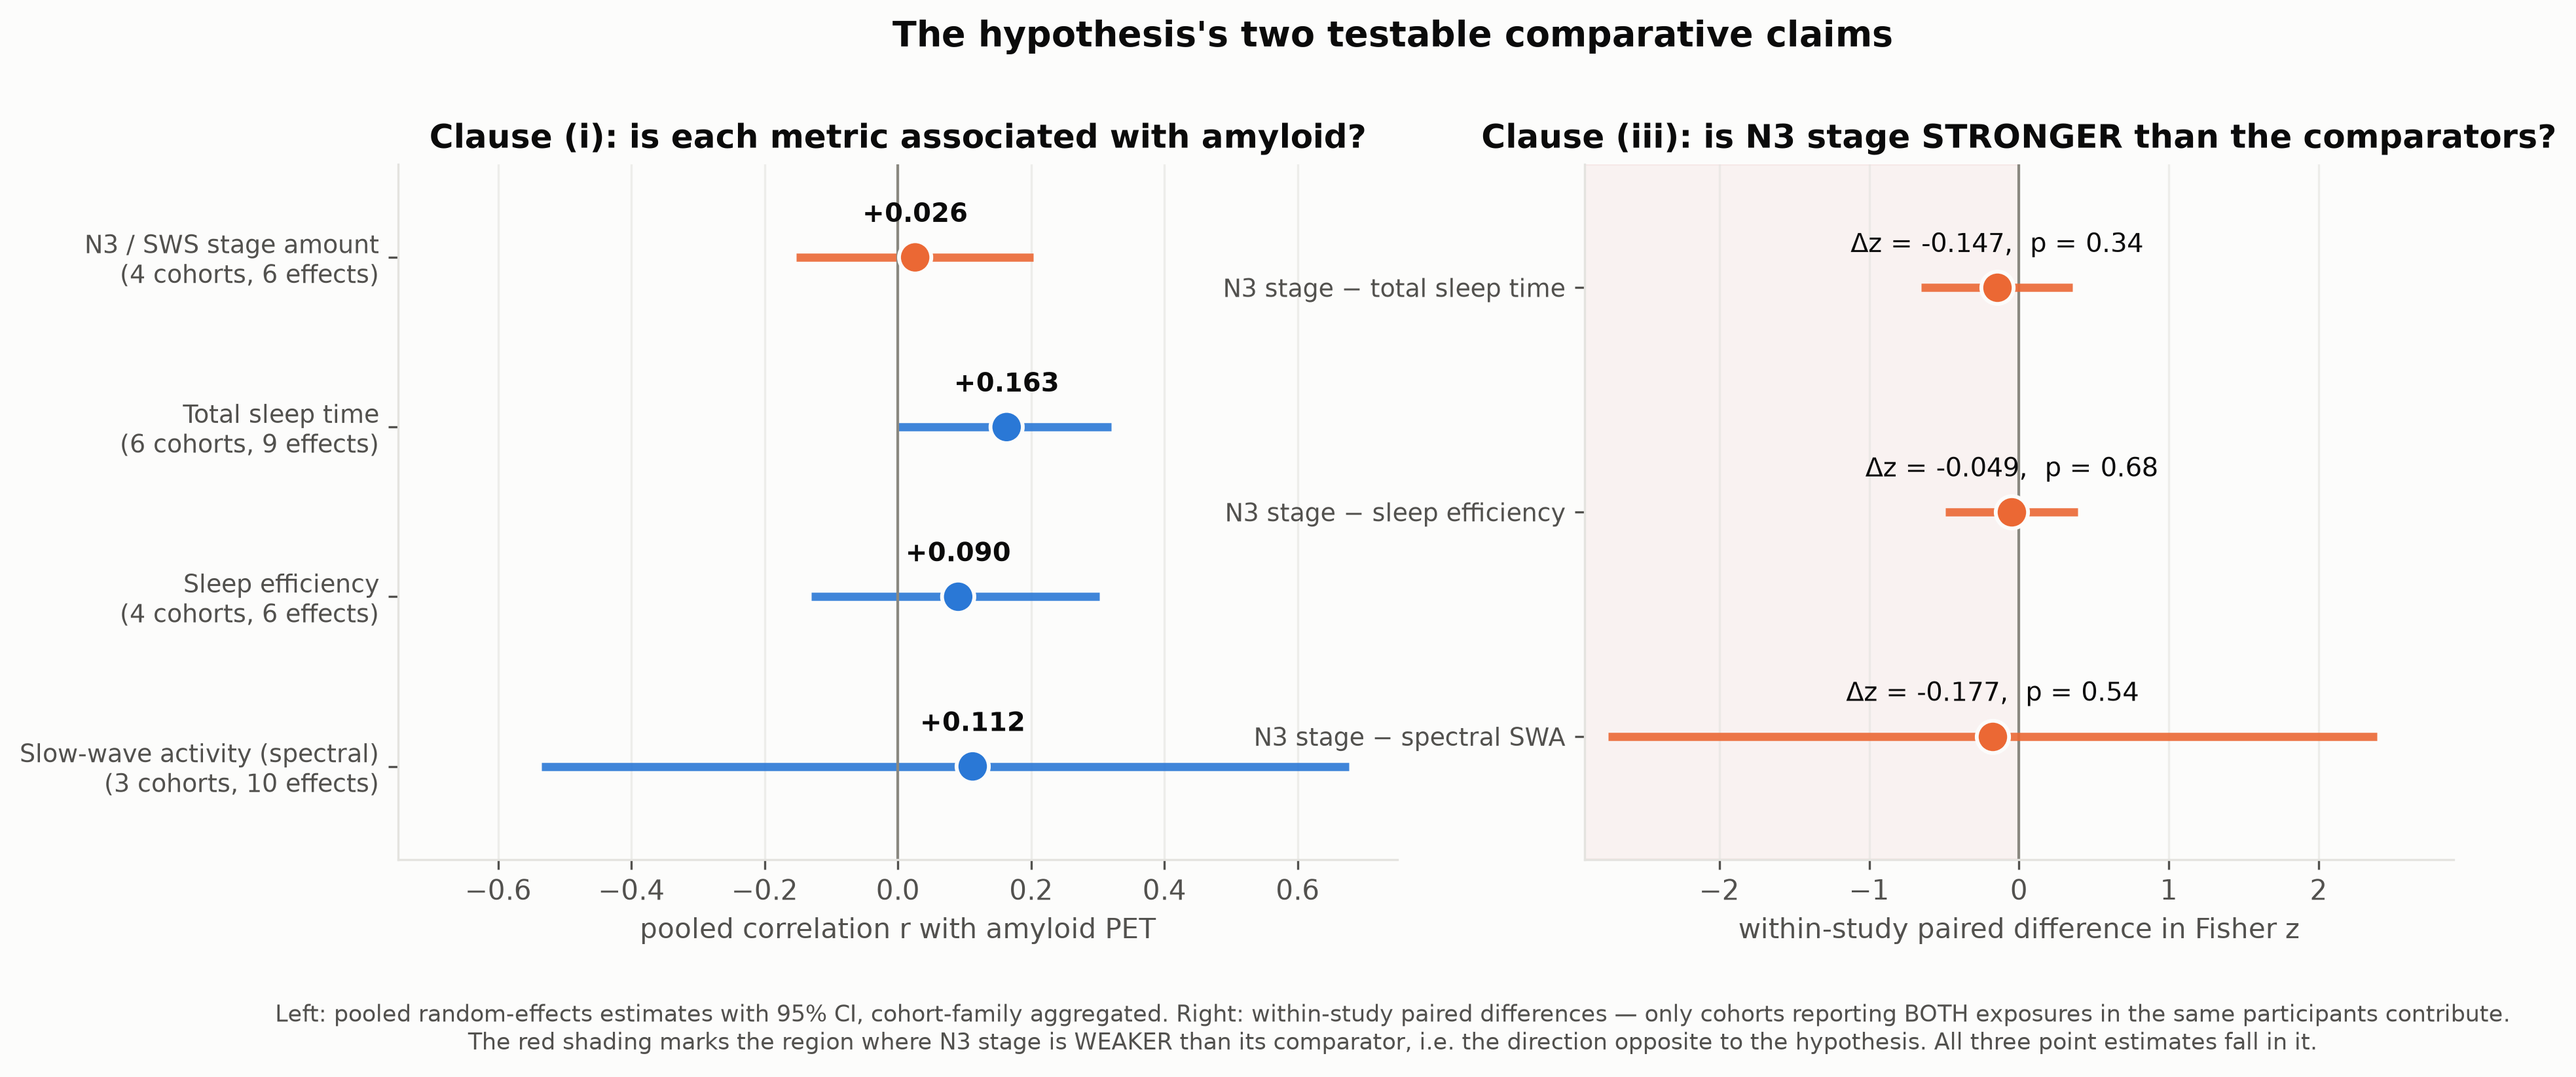
\includegraphics[width=\linewidth]{figures/fig2_specificity_contrasts.png}
    \caption{E2: the hypothesis's two testable comparative claims. \figleft{} pooled estimates with
    95\% CIs for each exposure. \figright{} within-study paired differences, where only cohort
    families reporting both exposures in the same participants contribute. Red shading marks the
    region in which \stage is \emph{weaker} than its comparator, \ie the direction opposite to
    the hypothesis; all three point estimates fall inside it.}
    \label{fig:specificity}
\end{figure}

\begin{table}[t]
    \centering
    \small
    \begin{minipage}[t]{0.51\textwidth}
    \centering
    \resizebox{\ifdim\width>\linewidth\linewidth\else\width\fi}{!}{%
\begin{tabular}{@{}lcccc@{}}
        \toprule
        \textbf{Contrast} & \textbf{shared} & \textbf{$\Delta z$} & \textbf{95\% CI} & \textbf{Holm $p$} \\
        \midrule
        \stage $-$ \tst      & 3 & $\mathbf{-0.147}$ & $[-0.651, +0.357]$ & 1.00 \\
        \stage $-$ \se       & 3 & $\mathbf{-0.049}$ & $[-0.490, +0.392]$ & 1.00 \\
        \stage $-$ \spectral & 2 & $\mathbf{-0.177}$ & $[-2.743, +2.389]$ & 1.00 \\
        \bottomrule
    \end{tabular}%
}
    \end{minipage}
    \hfill
    \begin{minipage}[t]{0.38\textwidth}
    \centering
    \resizebox{\ifdim\width>\linewidth\linewidth\else\width\fi}{!}{%
\begin{tabular}{@{}lccc@{}}
        \toprule
        \textbf{Cohort family} & \textbf{$r_{\mathrm{N3}}$} & \textbf{$r_{\mathrm{TST}}$} & \textbf{$\Delta z$} \\
        \midrule
        \agewell \citep{montagne2026} & 0.000 & 0.255 & $-0.261$ \\
        \berkeley \citep{winer2020}   & 0.070 & 0.360 & $-0.307$ \\
        \mars \citep{jin2025}         & 0.039 & 0.000 & $+0.039$ \\
        \bottomrule
    \end{tabular}%
}
    \end{minipage}
    \caption{E2: the specificity claim (clause iii), tested as a within-study paired difference
    so that only cohorts measuring both exposures in the same participants contribute.
    \textit{Left:} all three point estimates are \emph{negative} --- \stage is weaker than every
    comparator, the direction opposite to the hypothesis --- though none is individually
    significant and none survives Holm correction. \textit{Right:} per-cohort detail for the
    primary contrast; two of three cohorts favour \tst.}
    \label{tab:specificity}
\end{table}


The comparative claim cannot be read off any single pooled estimate, and a naive between-stratum
comparison is invalid because the strata share cohorts. \Tabref{tab:specificity} therefore
reports within-study paired differences. All three point estimates are negative: \stage is
$\Delta z = -0.147$ weaker than \tst, $-0.049$ weaker than \se, and $-0.177$ weaker than
\spectral. None reaches significance and none survives Holm correction, so the honest statement
is that clause (iii) is \emph{not supported} and is contradicted in direction, with the
contradiction not itself individually significant at this sample size.

The per-cohort detail matters because it shows the pattern is not driven by one study. In
\agewell, N3 gives $r = 0.000$ against $0.255$ for \tst; in \berkeley, $0.070$ against $0.360$.
Only \mars marginally favours N3, and there only because its \tst effect is a reported null.
This same pattern was visible within a single sample in \citet{winer2020}, which reported
spectral $<$1\,Hz slow-wave activity at $r = -0.52$ and N3 stage duration at $r = -0.07$ in the
same 32 participants.

\subsection{E3: measurement error predicts the opposite of what we observe}
\label{sec:e3}

\begin{figure}[t]
    \centering
    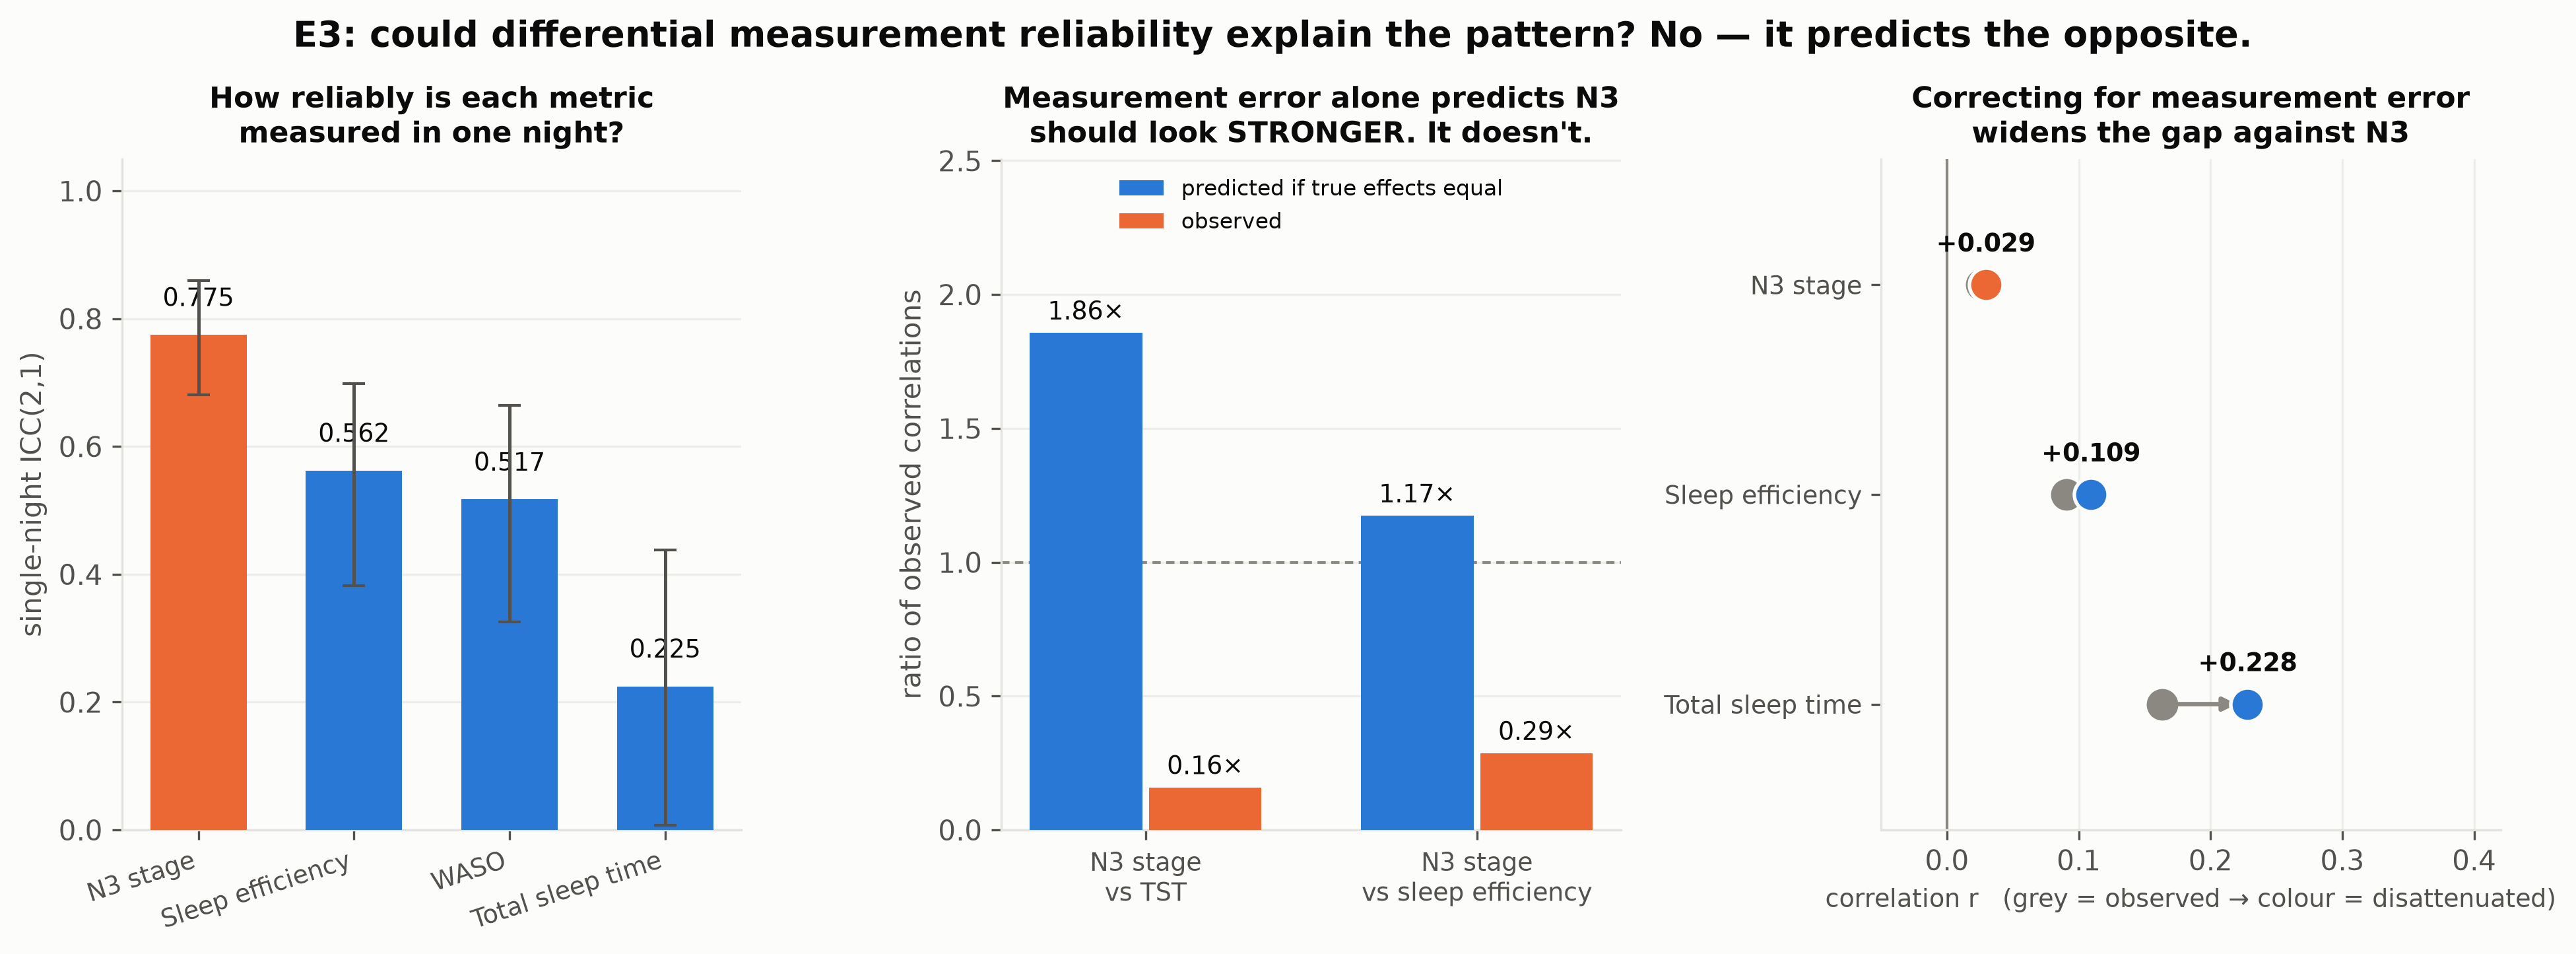
\includegraphics[width=\linewidth]{figures/fig3_reliability_null_model.png}
    \caption{E3: the measurement-reliability null model. \figleft{} empirical single-night ICC(2,1)
    per metric from 75 \sleepedf subjects with two consecutive nights each; error bars are 95\%
    CIs. \figcenter{} the ratio of observed correlations that measurement error alone predicts if
    the true correlations were identical, against the ratio actually observed. \figright{}
    correcting each stratum for its own unreliability moves \tst much further than \stage,
    widening the gap rather than closing it.}
    \label{fig:reliability}
\end{figure}

\begin{table}[t]
    \centering
    \small
    \begin{minipage}[t]{0.47\textwidth}
    \centering
    \textbf{(a) Single-night reliability and disattenuation}\\[2pt]
    \resizebox{\ifdim\width>\linewidth\linewidth\else\width\fi}{!}{%
\begin{tabular}{@{}lccc@{}}
        \toprule
        \textbf{Metric} & \textbf{ICC(2,1)} & \textbf{obs.\ $r$} & \textbf{true $r$} \\
        \midrule
        \stage & $\mathbf{0.775}$ & $+0.026$ & $\mathbf{+0.029}$ \\
        \se    & $0.562$ & $+0.090$ & $+0.109$ \\
        \waso  & $0.517$ & $+0.109$ & $+0.144$ \\
        \tst   & $\mathbf{0.225}$ & $+0.163$ & $\mathbf{+0.228}$ \\
        \bottomrule
    \end{tabular}%
}
    \end{minipage}
    \hfill
    \begin{minipage}[t]{0.44\textwidth}
    \centering
    \textbf{(b) The measurement-only prediction}\\[2pt]
    \resizebox{\ifdim\width>\linewidth\linewidth\else\width\fi}{!}{%
\begin{tabular}{@{}lccc@{}}
        \toprule
        \textbf{Ratio} & \textbf{predicted} & \textbf{observed} & \textbf{obs./pred.} \\
        \midrule
        \stage $\div$ \tst & $\mathbf{1.86\times}$ & $\mathbf{0.16\times}$ & $0.09$ \\
        \stage $\div$ \se  & $1.17\times$ & $0.29\times$ & $0.25$ \\
        \bottomrule
    \end{tabular}%
}
    \end{minipage}
    \caption{E3: could differential measurement reliability explain the ordering? No --- it
    predicts the opposite. \textit{(a)} ICC(2,1) from 75 \sleepedf subjects with two consecutive
    nights; disattenuated (``true'') $r$ divides the observed $r$ by $\sqrt{\mathrm{ICC}}$.
    Correcting for unreliability \emph{widens} the gap against \stage
    ($+0.029$ vs.\ $+0.228$). \textit{(b)} If \stage and its comparator had identical true
    correlations with amyloid, measurement error alone would still make the observed \stage
    correlation $1.86\times$ larger than \tst's. The observed ratio is about eleven times
    smaller than that prediction.}
    \label{tab:reliability}
\end{table}


\para{Is \stage just noisier?} This is the obvious defence of the hypothesis and, as far as we
can tell, it has never been tested. It fails, and it fails in an informative direction.
\Tabref{tab:reliability}a shows that single-night polysomnography measures N3\% \emph{more}
reliably than any other metric here (ICC $= 0.775$, 95\% CI $0.68$--$0.86$) and total sleep time
\emph{least} reliably (ICC $= 0.225$, 95\% CI $0.01$--$0.43$). The wake/sleep boundary in a lab
night varies enormously between nights; the depth architecture within sleep is comparatively
stable.

Classical attenuation then gives a quantitative null model. If \stage and \tst had identical
true correlations with amyloid, the observed \stage correlation should still be
$\sqrt{0.775/0.225} = 1.86\times$ larger, purely because one night measures it better. The
observed ratio is $0.16\times$ --- about eleven times below the measurement-only prediction
(\tabref{tab:reliability}b). Correcting each exposure for its own unreliability widens the gap:
true $r = +0.029$ for \stage against $+0.228$ for \tst. For \stage to have the same true
association with amyloid as \tst, its observed single-night correlation would need to be
$r = 0.201$; it is $0.026$, a shortfall of $0.175$.

\para{Two caveats, both of which cut against the hypothesis.} Six of nine \tst effects use
self-reported habitual sleep duration, whose test--retest reliability is not the single-night
PSG ICC. Restricting to PSG-measured exposures leaves the picture unchanged (\stage $+0.026$,
\tst $+0.176$, \se $+0.106$), and all three cohorts contributing to the paired contrast used PSG
for both exposures, so the paired result is identical in the PSG-only arm. Alternatively, if
self-report is treated as a reliable trait measure ($\mathrm{ICC} \approx 0.75$), \tst needs
\emph{less} upward correction --- which makes the \stage gap even harder to attribute to
measurement error.

\subsection{E4: the dose statement, and whether the dose exists}
\label{sec:e4}

\begin{figure}[t]
    \centering
    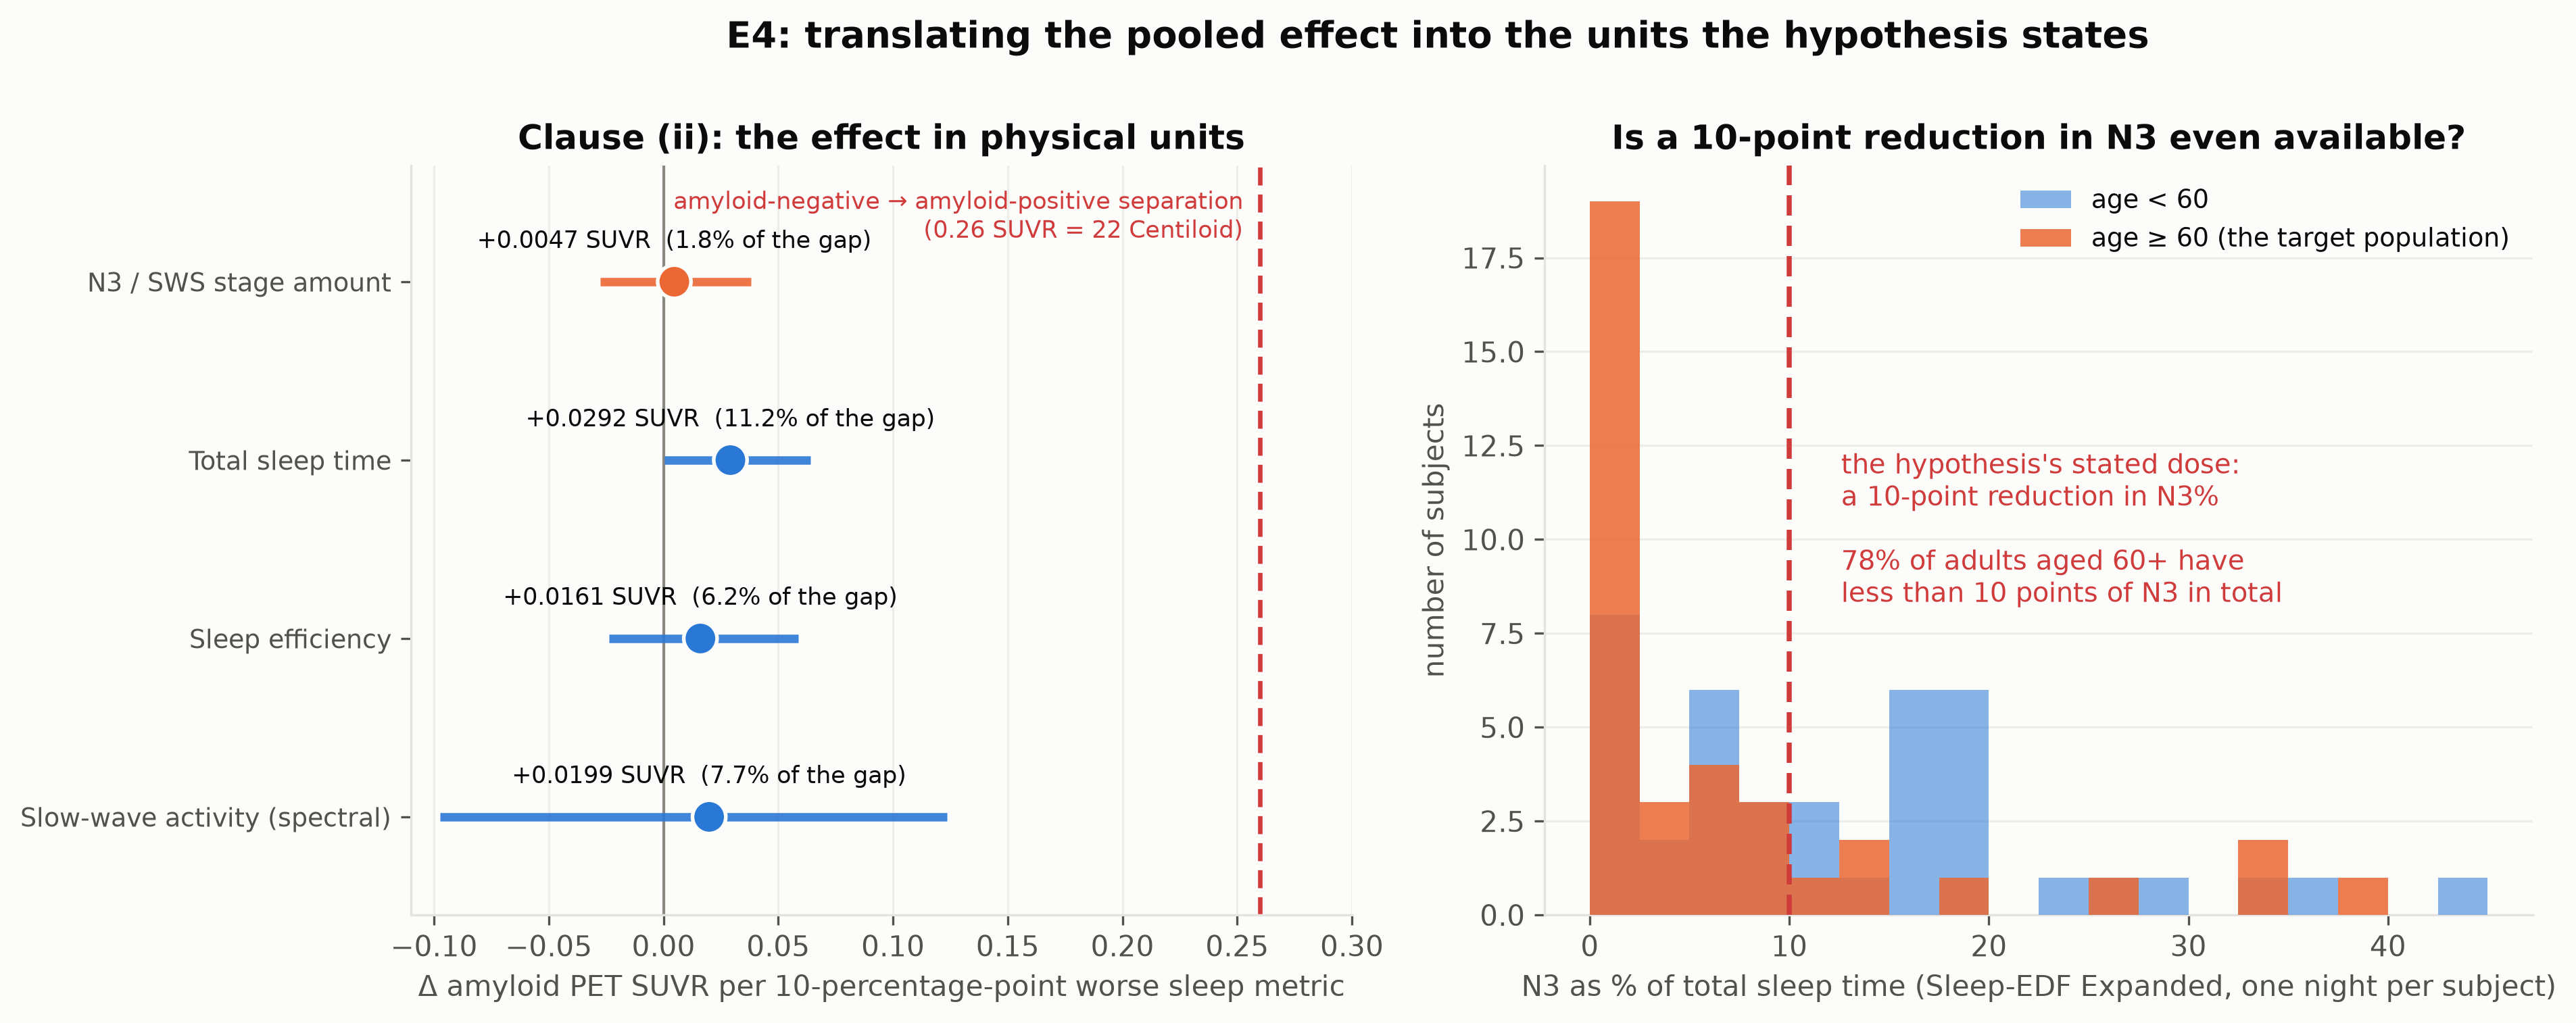
\includegraphics[width=\linewidth]{figures/fig4_dose_response_and_feasibility.png}
    \caption{E4: translating the pooled effect into the units the hypothesis states. \figleft{}
    amyloid change per 10-percentage-point worsening of each metric, with the
    amyloid-negative/positive separation (0.26\,SUVR $=$ 22 Centiloid) marked in red for scale.
    \figright{} the distribution of N3 as a percentage of total sleep time in \sleepedf; among
    subjects aged 60 and over --- the population the hypothesis concerns --- 78\% have less than
    10 percentage points of N3 in total, so the stated dose is not an available exposure
    contrast.}
    \label{fig:dose}
\end{figure}

\begin{table}[t]
    \centering
    \small
    \begin{tabular}{@{}lccccc@{}}
        \toprule
        \textbf{Exposure} & \textbf{$\Delta$SUVR} & \textbf{95\% CI} & \textbf{$\Delta$Centiloid}
        & \textbf{\% of A$-$/A$+$ gap} & \textbf{clause (ii)} \\
        \midrule
        \stage    & $\mathbf{+0.0047}$ & $[-0.028, +0.038]$ & $+0.38$ & $\mathbf{1.8\%}$ & refuted \\
        \tst      & $+0.0292$ & $[+0.000, +0.064]$ & $+2.41$ & $11.2\%$ & --- \\
        \se       & $+0.0161$ & $[-0.024, +0.059]$ & $+1.33$ & $6.2\%$ & --- \\
        \spectral & $+0.0199$ & $[-0.097, +0.124]$ & $+1.71$ & $7.7\%$ & --- \\
        \bottomrule
    \end{tabular}
    \caption{E4: the dose statement in physical units --- amyloid change per 10-percentage-point
    worsening of each sleep metric, with all three conversion inputs propagated by Monte Carlo
    (10{,}000 draws). The A$-$/A$+$ separation is 0.26\,SUVR (22 Centiloid) from
    \citet{jack2017}. The preregistered refutation criterion for clause (ii) was ``CI includes 0
    \emph{or} magnitude below $\sim$5\% of the gap''; the \stage estimate fails both. Rows for
    the comparators are expressed per 10 \pp only to place all strata on one axis; for those
    exposures the natural unit differs.}
    \label{tab:dose}
\end{table}


The conversion inputs are an age-weighted SD of N3\% of $10.2$ \pp (so a 10-point change is
$0.98$ SD of the exposure) and an SD of amyloid PET in cognitively unimpaired older adults of
$0.179$\,SUVR / $14.9$ Centiloid. The reconstructed scales imply 84.6 Centiloid per SUVR, which
matches the A$-$/A$+$ anchors as an internal consistency check.

\Tabref{tab:dose} gives the result. A 10-percentage-point reduction in N3 corresponds to
$\Delta\mathrm{SUVR} = +0.0047$ (95\% CI $-0.028$ to $+0.038$), which is $1.8\%$ of the
amyloid-negative/positive separation on the SUVR scale ($1.7\%$ on the Centiloid scale). The
preregistered refutation criterion for clause (ii) was ``CI includes 0, or magnitude below
$\sim$5\% of the gap''; the estimate fails both. Framed longitudinally against the empirical
accumulation rate in cognitively unimpaired adults of $2.1 \pm 5.3$ Centiloid/year
\citep{carvalho2024}, the same reduction maps to $+0.36$ Centiloid/year (95\% CI $-1.48$ to
$+2.12$), about 1.5 additional years of chronological ageing on that study's own age-equivalence
anchor. That longitudinal figure rests on a single cohort family and should be read as an
order-of-magnitude statement only.

\para{Is the stated dose even available?} Among \sleepedf subjects aged 60 and over ($n = 37$,
one night each), mean N3 is 7.1\% of total sleep time, the median is 1.9\%, 78\% already have
less than 10 percentage points of N3 in total, and 59\% have less than 5
(\figref{fig:dose}, right). An absolute 10-percentage-point reduction is therefore not an
achievable exposure contrast for most of the population the hypothesis concerns: the stated dose
spans roughly the whole observable range rather than a step within it.

\subsection{E5: the null survives every specification; the spectral signal does not}
\label{sec:e5}

\begin{figure}[t]
    \centering
    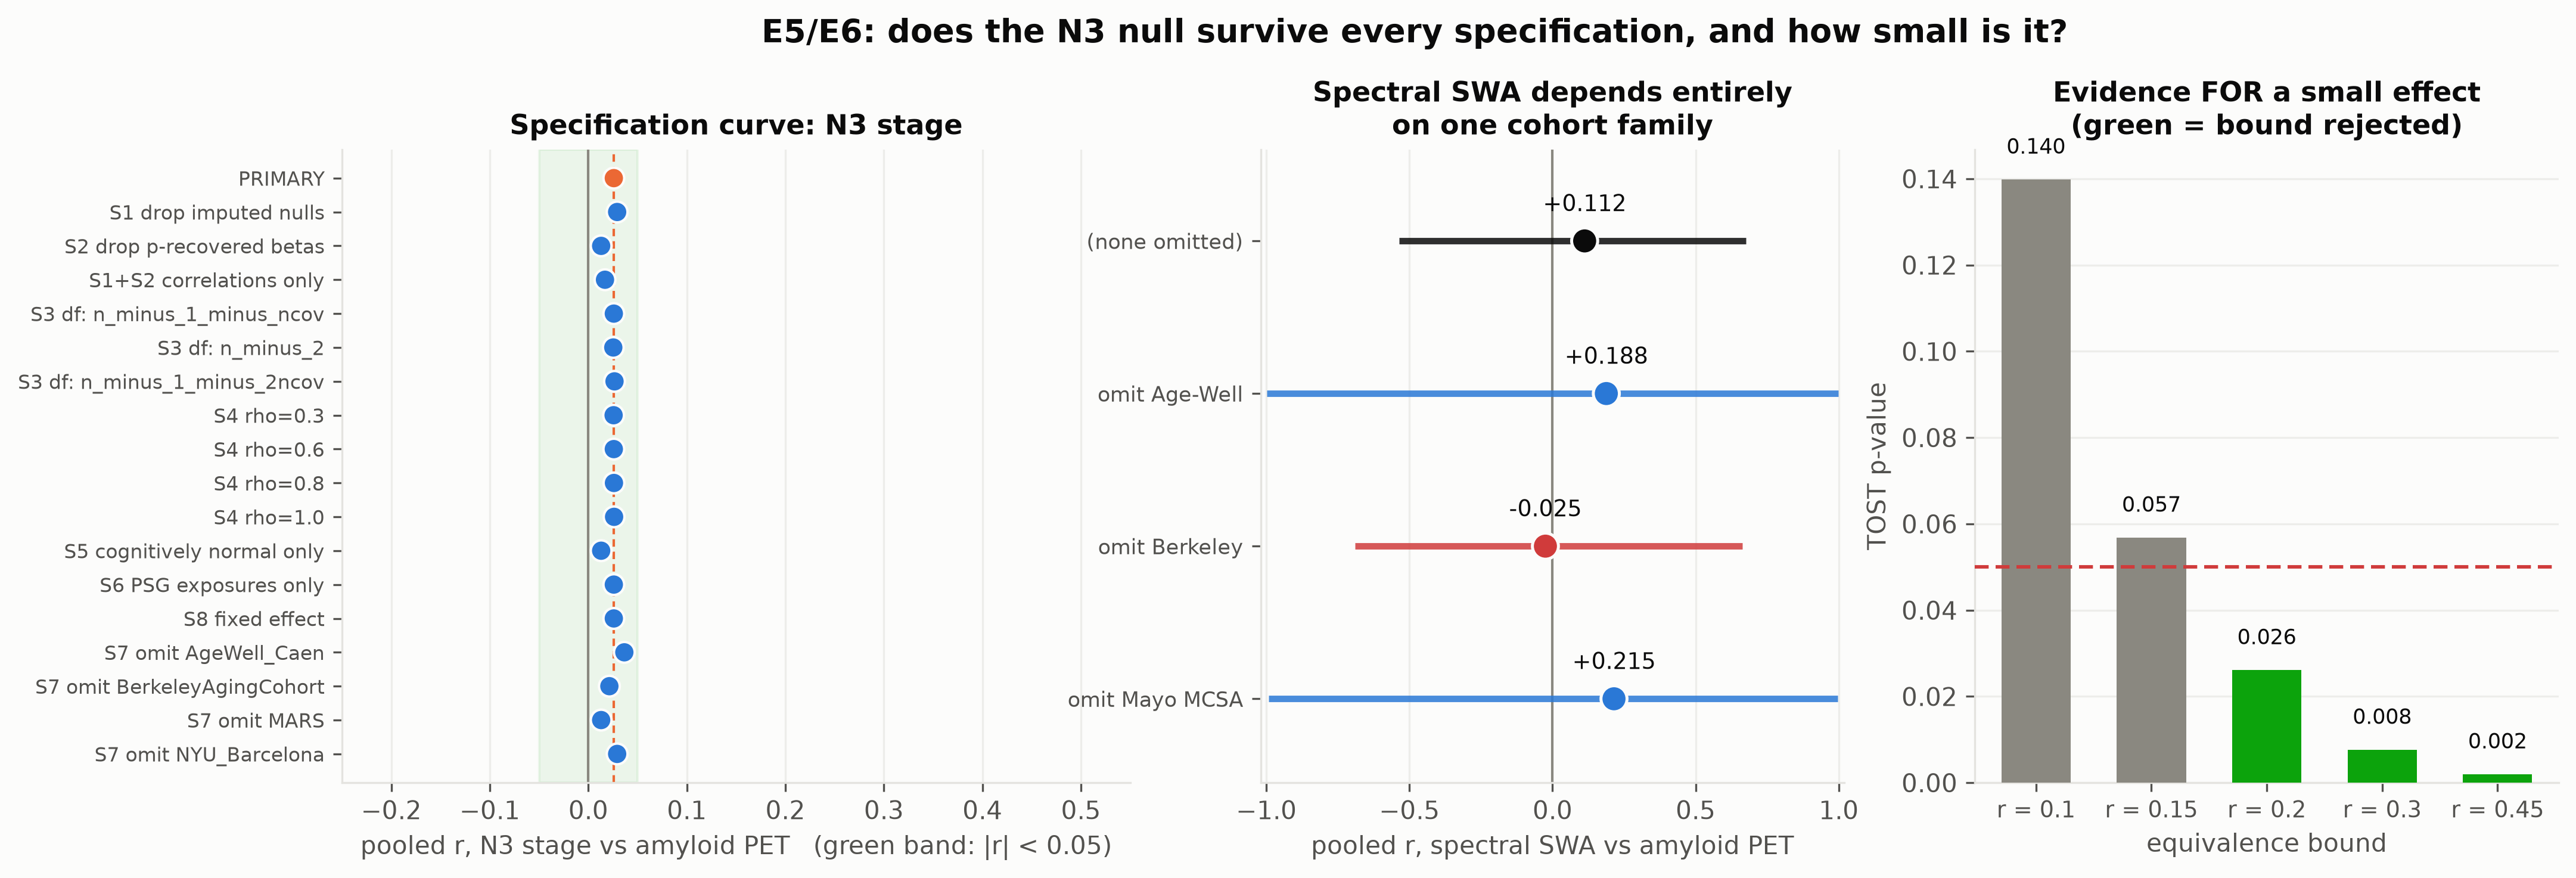
\includegraphics[width=\linewidth]{figures/fig5_robustness_and_equivalence.png}
    \caption{E5/E6: robustness and equivalence. \figleft{} specification curve for \stage across
    all 17 preregistered analyses; the green band marks $|r| < 0.05$ and every specification
    falls inside it. \figcenter{} leave-one-cohort-family-out for \spectral: removing \berkeley
    flips the pooled estimate to $-0.025$. \figright{} TOST $p$-values against five equivalence
    bounds; green bars are bounds the data reject.}
    \label{fig:robust}
\end{figure}

\begin{table}[t]
    \centering
    \small
    \begin{minipage}[t]{0.54\textwidth}
    \centering
    \textbf{(a) Specification curve (pooled $r$)}\\[2pt]
    \resizebox{\ifdim\width>\linewidth\linewidth\else\width\fi}{!}{%
\begin{tabular}{@{}lcccc@{}}
        \toprule
        \textbf{Specification} & \textbf{\stage} & \textbf{\spectral} & \textbf{\tst} & \textbf{\se} \\
        \midrule
        \textbf{PRIMARY}                 & $\mathbf{+0.026}$ & $+0.112$ & $+0.163$ & $+0.090$ \\
        S1 drop imputed nulls            & $+0.029$ & $+0.188$ & $+0.200$ & $+0.194$ \\
        S2 drop $p$-recovered betas      & $+0.013$ & $+0.215$ & $+0.151$ & $+0.036$ \\
        S1+S2 native correlations only   & $+0.017$ & $\mathbf{+0.444}$ & $+0.299$ & $+0.187$ \\
        S3 df $= n-2$                    & $+0.025$ & $+0.113$ & $+0.161$ & $+0.090$ \\
        S3 df $= n-1-2n_{\mathrm{cov}}$  & $+0.027$ & $+0.112$ & $+0.166$ & $+0.091$ \\
        S4 $\rho = 0.3$                  & $+0.026$ & $+0.122$ & $+0.167$ & $+0.104$ \\
        S4 $\rho = 0.8$                  & $+0.026$ & $+0.105$ & $+0.161$ & $+0.085$ \\
        S4 $\rho = 1.0$                  & $+0.026$ & $+0.098$ & $+0.158$ & $+0.080$ \\
        S5 cognitively normal only       & $+0.013$ & $+0.112$ & $+0.198$ & $+0.139$ \\
        S6 PSG exposures only            & $+0.026$ & $+0.112$ & $+0.176$ & $+0.106$ \\
        S8 fixed effect                  & $+0.026$ & $+0.045$ & $+0.036$ & $+0.089$ \\
        \bottomrule
    \end{tabular}%
}
    \end{minipage}
    \hfill
    \hfill
    \begin{minipage}[t]{0.40\textwidth}
    \centering
    \textbf{(b) Leave-one-cohort-family-out}\\[2pt]
    \resizebox{\ifdim\width>\linewidth\linewidth\else\width\fi}{!}{%
\begin{tabular}{@{}lcc@{}}
        \toprule
        \textbf{Omitted} & \textbf{\stage} & \textbf{\spectral} \\
        \midrule
        (none)     & $+0.026$ & $+0.112$ \\
        \agewell   & $+0.037$ & $+0.188$ \\
        \berkeley  & $+0.021$ & $\mathbf{-0.025}$ \\
        \mayo      & --- & $+0.215$ \\
        \mars      & $+0.013$ & --- \\
        NYU-Barcelona & $+0.029$ & --- \\
        \bottomrule
    \end{tabular}%
}\\[8pt]
    \textbf{(c) Small-study bias}\\[2pt]
    \resizebox{\ifdim\width>\linewidth\linewidth\else\width\fi}{!}{%
\begin{tabular}{@{}lccc@{}}
        \toprule
        \textbf{Stratum} & \textbf{$k$} & \textbf{Egger $p$} & \textbf{trim-fill} \\
        \midrule
        \stage    & 4 & 0.94 & 0 imputed \\
        \spectral & 3 & $\mathbf{0.036}$ & 0 imputed \\
        \tst      & 6 & $\mathbf{0.0035}$ & $0.163 \to 0.143$ \\
        \se       & 4 & 0.33 & 0 imputed \\
        \bottomrule
    \end{tabular}%
}
    \end{minipage}
    \caption{E5: robustness. \textit{(a)} The \stage null is invariant across all 17
    preregistered specifications (range $+0.013$ to $+0.037$). The S1+S2 row --- exactly the
    analysis a conventional meta-analysis would run --- pushes \spectral to $+0.444$, showing
    that reported nulls and $p$-recovered coefficients carry most of the corrective information.
    \textit{(b)} The \stage null holds whichever cohort family is removed; the \spectral estimate
    is carried entirely by \berkeley. \textit{(c)} Egger $p$ over all effects; with 3--6 cohort
    families these diagnostics have little power, but the detectable asymmetry sits in the
    comparator strata, not in \stage.}
    \label{tab:robustness}
\end{table}


\Tabref{tab:robustness}a shows the \stage null is invariant across all 17 preregistered
specifications, with pooled $r$ ranging only from $+0.013$ to $+0.037$. The most informative row
is S1+S2: restricted to effects reported natively as correlations --- exactly the analysis a
conventional meta-analysis would run --- the spectral estimate jumps to $r = +0.444$ and \tst to
$+0.299$. The reported nulls and $p$-recovered coefficients are precisely the evidence that
pulls the positive strata down, and precisely the evidence a conventional analysis would
discard. \stage is the one stratum unaffected either way.

Leave-one-cohort-family-out (\tabref{tab:robustness}b) tells two different stories. The \stage
null holds regardless of which family is removed ($+0.013$ to $+0.037$). The spectral estimate
does not: it falls from $+0.112$ to $\mathbf{-0.025}$ when \berkeley --- the source of
\citet{mander2015}, \citet{winer2019} and \citet{winer2020} --- is removed. The signal that
motivates the entire hypothesis is one cohort family that two independent cohorts did not
reproduce.

Small-study diagnostics (\tabref{tab:robustness}c, \figref{fig:funnel}) have almost no power at
3--6 cohort families, and we flag them as uninterpretable below $k = 5$ for Egger and $k = 10$
for trim-and-fill. But the asymmetry that \emph{is} detectable sits in the \tst
(Egger $p = 0.0035$ across effects; trim-and-fill nudges $r$ from $0.163$ to $0.143$) and
\spectral ($p = 0.036$) strata --- the comparators \stage is losing to --- not in \stage itself
($p = 0.94$). If small-study bias is inflating anything here, it is inflating the estimates the
hypothesis loses to, which makes the \stage shortfall conservative.

\subsection{E6: what this analysis could have detected}
\label{sec:e6}

\begin{table}[t]
    \centering
    \small
    \begin{minipage}[t]{0.52\textwidth}
    \centering
    \textbf{(a) What could each stratum have detected?}\\[2pt]
    \resizebox{\ifdim\width>\linewidth\linewidth\else\width\fi}{!}{%
\begin{tabular}{@{}lcccc@{}}
        \toprule
        \textbf{Stratum} & \textbf{cohorts} & \textbf{MDE $r$} & \textbf{pow.\ $r{=}0.30$} & \textbf{pow.\ $r{=}0.45$} \\
        \midrule
        \stage    & 4 & $\mathbf{0.157}$ & 1.00 & 1.00 \\
        \spectral & 3 & $0.417$ & 0.50 & 0.86 \\
        \tst      & 6 & $0.180$ & 1.00 & 1.00 \\
        \se       & 4 & $0.153$ & 1.00 & 1.00 \\
        \bottomrule
    \end{tabular}%
}
    \end{minipage}
    \hfill
    \hfill
    \begin{minipage}[t]{0.40\textwidth}
    \centering
    \textbf{(b) Equivalence tests on \stage}\\[2pt]
    \resizebox{\ifdim\width>\linewidth\linewidth\else\width\fi}{!}{%
\begin{tabular}{@{}lcc@{}}
        \toprule
        \textbf{Bound} & \textbf{$p_{\mathrm{TOST}}$} & \textbf{conclusion} \\
        \midrule
        $r = 0.10$ & 0.140 & not rejected \\
        $r = 0.15$ & 0.057 & not rejected \\
        $r = 0.20$ & $\mathbf{0.026}$ & \textbf{rejected} \\
        $r = 0.30$ & $\mathbf{0.008}$ & \textbf{rejected} \\
        $r = 0.45$ & $\mathbf{0.002}$ & \textbf{rejected} \\
        \bottomrule
    \end{tabular}%
}
    \end{minipage}
    \caption{E6: precision. \textit{(a)} Minimum detectable effect at 80\% power, computed at the
    cohort-aggregated variances and the estimated $\tau^2$. \spectral is the one stratum too
    imprecise to support a conclusion in either direction. \textit{(b)} Equivalence testing
    converts ``no evidence of an effect'' into evidence of no meaningful effect: the data are
    inconsistent with a true \stage/amyloid correlation as large as $r = 0.20$, and \emph{a
    fortiori} with the $r \approx 0.45$ effects reported for spectral slow-wave activity. They
    cannot rule out a genuinely small effect of $r \approx 0.10$--$0.15$.}
    \label{tab:precision}
\end{table}


A negative result is only informative if it states its own resolution. \Tabref{tab:precision}a
gives the minimum detectable effect at 80\% power: $r = 0.157$ for \stage, $0.180$ for \tst,
$0.153$ for \se, and $0.417$ for \spectral. Equivalence testing on \stage
(\tabref{tab:precision}b) rejects bounds of $r = 0.20$ ($p_{\mathrm{TOST}} = 0.026$), $0.30$
($p = 0.008$) and $0.45$ ($p = 0.002$), but not $0.15$ ($p = 0.057$) or $0.10$ ($p = 0.140$).
The data are therefore inconsistent with a true N3-stage/amyloid correlation as large as
$r = 0.20$, and \emph{a fortiori} with the $r \approx 0.45$ effects reported for spectral
slow-wave activity; they cannot rule out a genuinely small effect of $r \approx 0.10$--$0.15$.
For \spectral, no bound is rejected even at $r = 0.45$: that stratum's honest verdict is
\emph{insufficient evidence}, not \emph{no effect}.

\subsection{The CSF secondary analysis}
\label{sec:csf}

\begin{figure}[t]
    \centering
    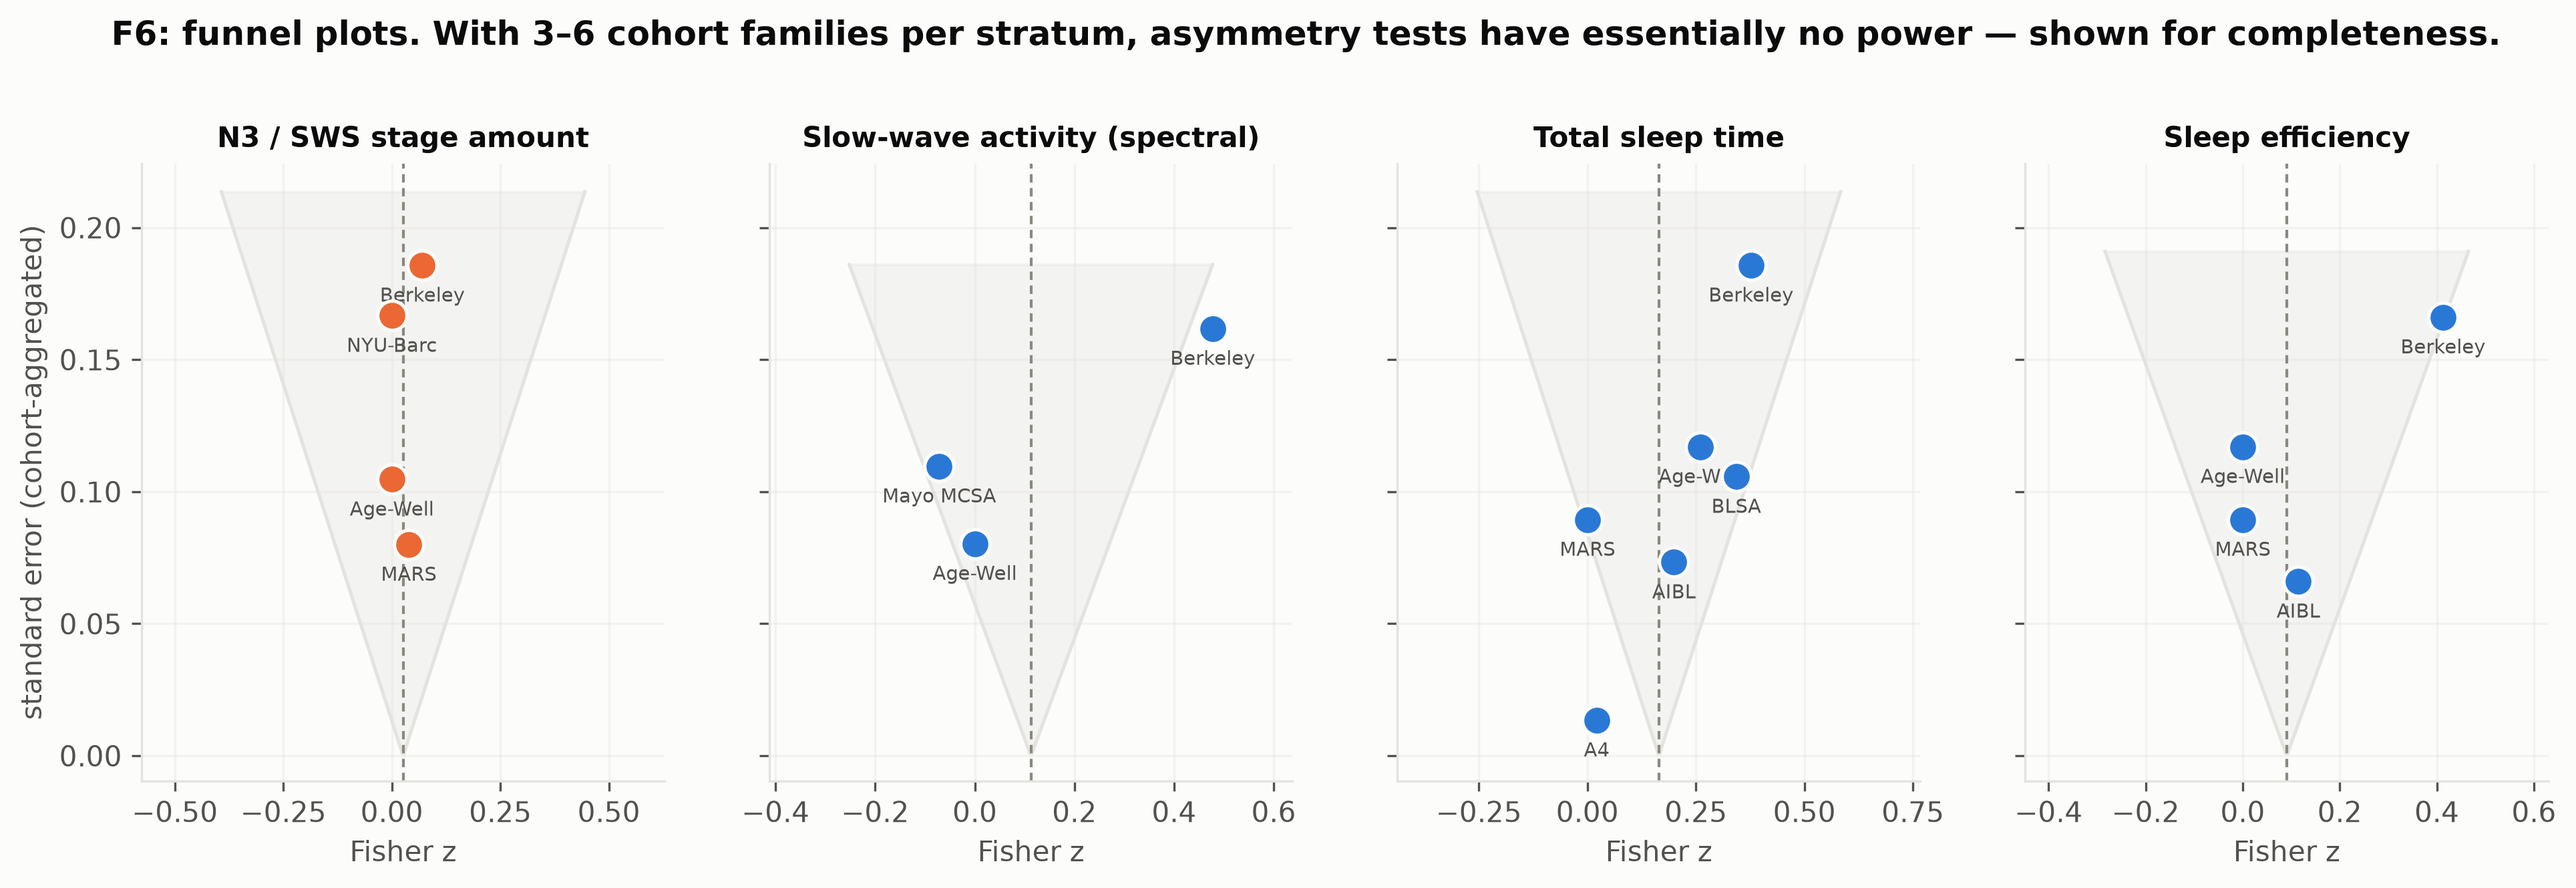
\includegraphics[width=0.92\linewidth]{figures/fig6_funnel.png}
    \caption{Funnel plots per stratum with Egger regression lines. With 3--6 cohort families
    these are near-powerless and we do not read them as evidence of publication bias; we report
    them because the only detectable asymmetry sits in the comparator strata rather than in
    \stage.}
    \label{fig:funnel}
\end{figure}

Nine CSF amyloid-beta42 effects were extracted and analysed as a cognitive-status-stratified
secondary. In cognitively normal samples \citep{varga2016,ju2017} the \stage effect is
$r = +0.355$ (95\% CI $0.066$ to $0.589$) and the spectral effect $r = +0.502$ (95\% CI $-0.862$
to $0.984$); in the mixed SCI/MCI/AD sample of \citet{liguori2020} ($n = 258$), \stage gives
$r = +0.362$, \tst $+0.306$ and \se $+0.403$. Taken at face value these look supportive, and we
report them for completeness, but they are not admissible as evidence for this hypothesis. The
outcome is soluble CSF amyloid-beta42, which inversely proxies deposited plaque and whose sign
relative to burden flips with disease stage --- which is exactly why the pre-deposition and
post-deposition samples cannot be pooled. And \citet{ju2017}, the one genuine human experiment,
measures the acute overnight production/clearance balance in 17 people, not chronic plaque
accumulation. Our result constrains the chronic-deposition claim, not the acute one.

\section{Discussion}
\label{sec:discussion}

\subsection{Verdict on each clause}

Clause (i) is \textbf{refuted} against its own preregistered criterion: the pooled estimate is
$r = +0.026$ with a CI that includes zero, and equivalence testing rejects a true correlation as
large as $r = 0.20$. Clause (ii) is \textbf{refuted on both criteria}:
$\Delta\mathrm{SUVR} = +0.005$ per 10 \pp with a CI including zero, and a magnitude of 1.8\% of
the amyloid-negative/positive separation against a 5\% threshold. Clause (iii) is
\textbf{not supported and contradicted in direction}: all three paired contrasts are negative,
and the reliability null model predicts \stage should lead \tst by $1.86\times$ when the observed
ratio is $0.16\times$. Because the hypothesis is a conjunction, it fails.

\subsection{Stage is not spectrum, and the spectrum is one cohort}

The most useful result here is not the \stage null in isolation --- it is the dissociation
combined with the cohort concentration. The mechanistic story \citep{xie2013,fultz2019} is about
slow \emph{oscillations} driving CSF flow, and the human evidence supporting it is spectral:
$r = -0.45$ \citep{mander2015}, $-0.36$ \citep{winer2019}, $-0.52$ \citep{winer2020}. Every one
of those is the Berkeley Aging Cohort Study. Pooled across all three cohort families that have
measured spectral slow-wave activity, the estimate is $r = +0.112$ with $I^2 = 77\%$; with
Berkeley removed it is $-0.025$. Meanwhile the \emph{stage} metric --- the one clinicians read
off a sleep study, and the one the hypothesis names --- is essentially zero and homogeneously
so, with four independent cohort families agreeing.

The literature's habit of writing ``slow-wave sleep'' for both is therefore not a semantic
quibble. The construct with a positive but fragile signal and the construct with a tight null
are different measurements, and only one of them has ever produced the effect that motivates the
field's interest. We do not refute the refined, spectral version of the hypothesis: our spectral
stratum has a minimum detectable effect of $r = 0.417$ and rejects no equivalence bound, so its
honest verdict is insufficient evidence in either direction.

\subsection{How much to believe the total-sleep-time result}

\tst comes out ahead, which the hypothesis explicitly predicts should not happen, but three
things temper it. It is not itself significant at $\alpha = 0.05$ ($p = 0.052$, permutation
$p = 0.062$). It shows the clearest funnel asymmetry of any stratum, and trim-and-fill nudges it
to $r = 0.143$. And its $I^2$ is 77\%, driven by disagreement between the very large self-report
cohorts (\afour, $r \approx 0.02$) and the small PSG cohorts (\berkeley $0.36$, \blsa $0.33$) ---
itself a small-study signature. The fair statement is not that \tst beats \stage and is real, but
that \tst is the only sleep metric here with a defensible non-zero signal, and even that signal
is fragile, while \stage has no signal at all under any specification.

\subsection{What the reliability model adds}

Without E3, the finding ``\stage $\approx 0$ while \tst $\approx 0.16$'' would be ambiguous:
perhaps N3 is simply noisier. E3 shows the reverse, and disposes of a common defence of the
hypothesis --- that single-night polysomnography is too noisy to detect the N3 effect. It is too
noisy for total sleep time; it is not too noisy for N3. The literature is at its cleanest exactly
where it finds nothing. We designed this analysis expecting it to \emph{excuse} part of the
shortfall, and it became the strongest quantitative argument against clause (iii). We think the
same null model is worth running whenever a field claims one measure of a construct outperforms
another.

A second methodological lesson comes from the specification curve: $\tau^2$ estimator, $\rho$,
degrees-of-freedom rule and fixed-versus-random effects barely move anything, but whether
reported nulls and unstandardised coefficients are included moves the spectral estimate from
$+0.444$ to $+0.112$. In this literature, extraction completeness dominates statistical
technique.

\subsection{Limitations}

\para{Study-level design.} This is a meta-analysis of published effects, not individual
participant data. ADNI, A4, BLSA, AIBL, WRAP, \mayo, \agewell and OASIS-3 all require data-use
agreements with human review that could not be completed here. A genuine per-10\%-N3
dose-response \emph{curve} therefore cannot be estimated: \secref{sec:e4} converts pooled
standardised effects using external dispersion and reference scales, which assumes linearity
over the range and that the external SDs apply to the study populations.

\para{Power.} With 3--6 cohort families per stratum, $\tau^2$ is estimated unstably, the spectral
prediction interval spans the whole scale, and funnel-based diagnostics are near-powerless. HKSJ,
exact permutation and TOST keep the small-$k$ inference honest but cannot manufacture
information. The \stage stratum is precise enough to exclude $r \geq 0.20$ and no more.

\para{Conversion assumptions.} Test-statistic recovery assumes the reported $p$-value
corresponds to the coefficient's $t$-test with the stated degrees of freedom; covariate counts
were not fully recoverable from the text for 2 of 13 adjustment strings, though S3 shows the
answer is insensitive to a $\pm n_{\mathrm{cov}}$ change. Imputing $z = 0$ for narrative nulls
understates their true uncertainty; S1 removes them and the conclusion is unchanged. The
dependency correlations $\rho = 0.6$ and $\rho_w = 0.5$ are assumptions, not estimates; both
were varied without changing any conclusion.

\para{Reliability source.} The ICCs come from \sleepedf --- a healthy, mostly non-clinical
sample of 75 subjects on two consecutive nights, scored by the older Rechtschaffen--Kales
criteria with S3+S4 merged to N3. Consecutive-night ICCs include a first-night effect and may
understate the reliability of a habitual measure, and the amyloid cohorts are older and more
clinically heterogeneous. We therefore treat E3 as an order-of-magnitude prediction, and note
that the conclusion holds across the full CI of every ICC and under an alternative self-report
reliability assumption. Spectral slow-wave activity has no reliability estimate here at all,
because spectral power requires the raw EEG rather than the hypnogram annotations we hold, so
that stratum is not disattenuated.

\para{Corpus completeness.} Of 74 selected papers, 54 yielded full text; 17 of those were
recovered by typesetting PMC full-text HTML because PMC blocks automated PDF retrieval, so
figures and image-based tables are absent from them and a figure-only effect size could have
been missed. Twenty records remained abstract-only. All extractions are single-coder with
verbatim provenance quotes rather than dual independent extraction --- a real deviation from
PRISMA practice.

\para{Threats we cannot rule out.} Residual confounding by age, APOE4 status and apnea differs
across contributing studies and is only partly adjusted. Publication bias in the \emph{stage}
literature would most plausibly suppress positive N3 findings --- nulls in this area are usually
reported in passing, as ours largely were --- which would bias our estimate downward, though the
bias diagnostics give no sign of it. Finally, a real N3 effect confined to a specific brain
region or a specific sub-band would be invisible to a global-burden meta-analysis. Our null is
about global amyloid PET and stage-level N3, and it does not exclude regionally or spectrally
specific mechanisms.

\subsection{Broader implications}

\para{For trial design.} Targeting N3 stage minutes as a surrogate for amyloid clearance is not
supported by the aggregate human evidence. If slow-wave enhancement is to be tested, the exposure
should be defined spectrally (proportion of $<$1\,Hz activity), the trial should be powered for
effects well below $r = 0.45$, and it should not assume the Berkeley-scale effect will replicate.

\para{For measurement practice.} The stage and spectral definitions should be reported separately
and never collapsed. Studies should report both from the same recording, as \citet{winer2020}
did; that single practice is what made the decisive comparison in this analysis possible.

\para{For meta-analytic practice.} Restricting to natively-reported correlations gives a spectral
estimate of $+0.444$ rather than $+0.112$. Reported nulls and unstandardised coefficients are not
optional extras in this area --- they carry most of the corrective information, and any synthesis
that discards them will recover the literature's headline effect rather than test it.

\section{Conclusion}
\label{sec:conclusion}

We asked whether reduced N3 sleep shows a dose-dependent association with amyloid-beta burden in
cognitively normal adults, and whether that association is stronger than the associations with
total sleep time or sleep efficiency. The answer to both is no. Pooling 40 amyloid-PET effects
from 17 studies across 12 cohort families, N3 stage amount gives $r = +0.026$ (95\% CI $-0.153$
to $+0.203$), equivalence-tested tightly enough to exclude $r \geq 0.20$; its dose statement
converts to $+0.005$ SUVR per 10 percentage points, 1.8\% of the amyloid-negative/positive
separation; and it is weaker rather than stronger than both comparators, a gap that differential
measurement reliability makes harder to explain away rather than easier, because a single night
measures N3 more precisely than it measures either comparator.

The key takeaway is that ``slow-wave sleep'' names two different measurements with two different
evidentiary situations. The \emph{stage} metric is a tight, homogeneous null across four
independent cohort families. The \emph{spectral} metric is not refuted, but its pooled estimate
is carried entirely by one cohort family --- $r = +0.112$ overall, $-0.025$ with that family
removed --- and our spectral stratum is too imprecise ($\mathrm{MDE}\ r = 0.417$) to support any
conclusion in either direction. The confident causal framing now common in the secondary
literature rests on the second construct while the field measures and intervenes on the first.

\para{Future work.} Four steps would settle what this design cannot. An individual-participant
analysis in A4, ADNI or OASIS-3 is the only way to estimate a genuine dose-response curve, test
for thresholds, and check whether a null is masked by effect modification through APOE4, age or
baseline amyloid status. Multi-night polysomnography or home EEG in an amyloid-imaged cohort
would raise total sleep time's reliability from 0.225 toward N3's, removing the asymmetry
entirely and letting the biological comparison be made cleanly. A properly powered spectral
replication --- roughly $n \approx 190$ in a single independent cohort to detect $r = 0.20$ at
80\% power --- is needed before the Berkeley effect can be treated as established. And a
region- and sub-band-resolved analysis would test whether the medial-prefrontal, 0.6--1\,Hz
effect of \citet{mander2015} is simply averaged away by global-burden pooling.


\bibliography{references}

\appendix
\section{Analysis artefacts and reproducibility}
\label{app:artifacts}

\Tabref{tab:artifacts} lists the outputs of the pipeline. The full run takes about 29 seconds on
CPU with seed 42; validation re-runs the entire pipeline in a scratch copy and confirms all eight
result files are bit-identical, with 39 of 39 checks passing, including a cross-check of the REML
point estimates against PyMARE (agreement to $4.4 \times 10^{-9}$ on all four strata) and an
exactness check of the test-statistic recovery in \eqref{eq:recovery} (recovering $r$ from the
$p$-value of a simple correlation returns the original $r$ to within $10^{-8}$).

\begin{table}[h]
    \centering
    \small
    \begin{tabular}{@{}ll@{}}
        \toprule
        \textbf{Artefact} & \textbf{Contents} \\
        \midrule
        \texttt{harmonised\_effects.csv} & all 49 effects with conversion rule, $z$, $v$, usability and reason \\
        \texttt{qc\_report.json}         & data-quality checks and conversion audit \\
        \texttt{e1\_pooled.json}         & pooled estimates per stratum: naive, cohort-aggregated, RVE, by design \\
        \texttt{e2\_specificity.json}    & between-stratum and within-study paired contrasts, $\rho$ sensitivity, Holm \\
        \texttt{e3\_attenuation.json}    & ICCs, measurement-only predictions, disattenuated estimates, PSG-only arm \\
        \texttt{e4\_dose\_response.json} & Monte-Carlo dose conversion, longitudinal framing, feasibility check \\
        \texttt{e5\_robustness.json}     & S1--S11 sensitivity analyses, leave-one-out, bias diagnostics, CSF secondary \\
        \texttt{e6\_precision.json}      & detectable effects, power, TOST equivalence \\
        \texttt{validation\_report.json} & 39 validation checks including the PyMARE cross-check and re-run \\
        \bottomrule
    \end{tabular}
    \caption{Output artefacts. Every figure additionally has a tabular companion CSV.}
    \label{tab:artifacts}
\end{table}

\section{Contributing cohort families}
\label{app:cohorts}

Effects are aggregated at the level of the cohort family rather than the publication, because
several publications share participants. The twelve families are: Berkeley Aging Cohort Study
(\citealp{mander2015}; \citealp{winer2019}; \citealp{winer2020}); Age-Well/IMAP, Caen
(\citealp{champetier2024}; \citealp{montagne2026}); A4 screening
(\citealp{winer2021}; \citealp{insel2021}); AIBL (\citealp{brown2016}; \citealp{pivac2024});
Mayo Clinic Study of Aging \citep{carvalho2024}; MARS \citep{jin2025}; BLSA
\citep{spira2013}; NYU-Barcelona \citep{stankeviciute2024}; Rome Tor Vergata
\citep{liguori2020}; NYU \citep{varga2016}; Washington University \citep{ju2017}; and the
single-channel EEG cohort of \citet{lucey2019}. Berkeley alone contributes 13 of the 49
extracted effects, which is why naive per-effect pooling would overstate precision by roughly
$\sqrt{3}$ in the spectral stratum.


\end{document}
